\documentclass[11pt,a4paper]{article}

\usepackage[T1]{fontenc}
\usepackage[utf8]{inputenc}
\usepackage{mathptmx}
\usepackage[scaled=0.9]{helvet}
% --- localización manual (babel-spanish no disponible en esta distribución)
\renewcommand{\contentsname}{Índice}
\renewcommand{\appendixname}{Apéndice}
\renewcommand{\figurename}{Figura}
\renewcommand{\tablename}{Cuadro}
\renewcommand{\refname}{Referencias}
\usepackage[margin=2.4cm]{geometry}
\usepackage{amsmath,amssymb,amsthm,mathtools}
\usepackage{booktabs}
\usepackage{tikz}
\usetikzlibrary{arrows.meta,calc,positioning,patterns,decorations.pathreplacing}
\usepackage{microtype}
\usepackage{enumitem}
\usepackage{tcolorbox}
\usepackage[hidelinks]{hyperref}
\usepackage{fancyhdr}
\usepackage{caption}

\tcbuselibrary{skins,breakable}

\captionsetup{font=small,labelfont=bf}

\pagestyle{fancy}
\fancyhf{}
\fancyhead[L]{\footnotesize Modelo matemático · Vision Rover Challenge}
\fancyhead[R]{\footnotesize\thepage}
\renewcommand{\headrulewidth}{0.4pt}

% ---------------------------------------------------------------- entornos
\newtheorem{teorema}{Teorema}[section]
\newtheorem{proposicion}[teorema]{Proposición}
\newtheorem{lema}[teorema]{Lema}
\newtheorem{corolario}[teorema]{Corolario}
\theoremstyle{definition}
\newtheorem{definicion}[teorema]{Definición}
\newtheorem{observacion}[teorema]{Observación}
\newtheorem{ejemplo}[teorema]{Ejemplo}

\newenvironment{demo}{\par\noindent\textit{Demostración.}\;}{\hfill$\blacksquare$\par\medskip}

\newtcolorbox{resultado}[1][]{
  enhanced, breakable, colback=black!3, colframe=black!55,
  boxrule=0.5pt, arc=1pt, left=6pt, right=6pt, top=5pt, bottom=5pt, #1}

% ---------------------------------------------------------------- macros
\newcommand{\R}{\mathbb{R}}
\newcommand{\Rot}{\mathbf{R}}
\newcommand{\uu}{\mathbf{u}}
\newcommand{\vv}{\mathbf{v}}
\newcommand{\nn}{\mathbf{n}}
\newcommand{\dd}{\mathbf{d}}
\newcommand{\cc}{\mathbf{c}}
\newcommand{\pp}{\mathbf{p}}
\newcommand{\qq}{\mathbf{q}}
\newcommand{\NN}{\mathbf{N}}
\newcommand{\ww}{\mathbf{w}}
\newcommand{\ee}{\mathbf{e}}
\newcommand{\gv}{\mathbf{g}}
\DeclareMathOperator*{\argmin}{arg\,min}
\DeclareMathOperator*{\argmax}{arg\,max}
\newcommand{\aaa}{\mathbf{a}}
\newcommand{\cross}[2]{#1 \wedge #2}
\newcommand{\dif}{\operatorname{d}\!}
\newcommand{\atantwo}{\operatorname{atan2}}
\newcommand{\conv}{\operatorname{conv}}
\newcommand{\intr}{\operatorname{int}}
\newcommand{\diam}{\operatorname{diam}}
\newcommand{\sgn}{\operatorname{sgn}}
\newcommand{\celda}{\mathrm{c}}
\newcommand{\grados}{^{\circ}}

\begin{document}

% ================================================================ PORTADA
\begin{titlepage}
\centering
\vspace*{2.2cm}
{\Large\scshape Universidad Hispanoamericana}\\[0.2cm]
{\large Ingeniería Mecatrónica}\\[2.4cm]

\rule{\linewidth}{1.2pt}\\[0.45cm]
{\LARGE\bfseries Modelo matemático para la detección, localización\\[0.18cm]
y planificación geométrica del transporte\\[0.18cm]
de objetos cúbicos}\\[0.45cm]
\rule{\linewidth}{1.2pt}\\[0.9cm]

{\large Formalización del motor de visión artificial del \textit{Vision Rover Challenge},\\
estimación de pose de cuadrados y capa geométrica de planificación de rutas}\\[2.6cm]

\begin{tabular}{rl}
\textbf{Autor} & Sebastián Vega Amores\\[0.15cm]
\textbf{Repositorio base} & \texttt{Universidad-Cenfotec/Vision-Rover-Challenge}\\[0.15cm]
\textbf{Protocolo de telemetría} & v1 (TCP/NDJSON, puerto 2026)\\[0.15cm]
\textbf{Fecha} & 3 de septiembre de 2026 (rev. 3)\\
\end{tabular}

\vfill
{\small Documento técnico. Todas las magnitudes numéricas citadas provienen del repositorio
oficial (\texttt{reglamento.md}, \texttt{el\_reto.md}, \texttt{robot.md},
\texttt{vision-system/}) y se identifican con su origen en el cuadro maestro de
parámetros de la sección \ref{sec:parametros}.}
\end{titlepage}

\tableofcontents
\newpage

% ================================================================ 0
\section{Alcance, hipótesis y trazabilidad}

\subsection{Qué resuelve este documento}

Se construye el aparato matemático necesario para tres problemas encadenados:

\begin{enumerate}[label=(\Roman*),leftmargin=2.2em]
\item \textbf{Formalizar el motor de visión.} Describir con precisión qué magnitud
      física estima cada etapa del sistema oficial, mediante qué transformación, y
      con qué error acotado. Sin esto no es posible saber qué significa un número
      del contrato ni cuánta confianza merece.
\item \textbf{Modelar el objeto cuadrado.} Determinar la posición exacta y el ángulo
      de inclinación de un cubo a partir de evidencia geométrica parcial, y
      reconstruir sus cuatro vértices. Se desarrollan dos familias de estimadores:
      el ajuste robusto de silueta (que es el que implementa el motor oficial) y la
      familia analítica por vértices, cerrada en forma exacta.
\item \textbf{Planificar geométricamente el transporte.} Derivar los lugares
      geométricos de aproximación, contacto y empuje; el embudo de tolerancia que
      decide si un empuje es viable; y el costo de una ruta como funcional sobre el
      plano.
\end{enumerate}

\subsection{Qué queda deliberadamente fuera}

Por decisión de alcance, este documento \emph{no} desarrolla: la síntesis del
controlador de bajo nivel (PID de rumbo, control de giro por giróscopo), la fusión
sensorial (IMU, ultrasónico, infrarrojo, sensor de color), la asignación
multi-agente de tareas, ni el protocolo de coordinación entre rovers. Cuando la
geometría impone una condición que esas capas deben satisfacer, la condición se
enuncia como \emph{restricción de interfaz} y se marca como tal.

\subsection{Hipótesis de trabajo}
\label{sec:hipotesis}

\begin{enumerate}[label=H\arabic*.,leftmargin=2.6em,itemsep=3pt]
\item \textbf{Planitud.} La superficie de juego es un plano. Los marcadores de esquina,
      las bases de los cubos y las ruedas del rover pertenecen a ese plano.
\item \textbf{Cámara fija y calibrada.} Durante una ronda la cámara no se mueve; la
      distorsión radial ya fue rectificada y los intrínsecos efectivos corresponden a
      la imagen rectificada.
\item \textbf{Proyección central.} La cámara es un modelo estenopeico con centro
      óptico $C$ a altura $H$ sobre el plano de juego.
\item \textbf{Rigidez y dimensiones conocidas.} El cubo es un sólido rígido de arista
      $L$ conocida; el rover es un cuerpo rígido de ancho $W$ y largo $\Lambda$
      conocidos.
\item \textbf{Cuasiestática.} En el empuje, las velocidades son suficientemente bajas
      para despreciar efectos inerciales sobre el objeto.
\item \textbf{Contacto plano.} El cubo no vuelca ni se levanta: su base permanece en
      contacto con el plano, de modo que su configuración vive en $SE(2)$.
\end{enumerate}

\subsection{Trazabilidad de las magnitudes}

Toda constante numérica utilizada más adelante aparece en el cuadro maestro
(sección \ref{sec:parametros}) con tres atributos: valor, unidad y \emph{origen}
(archivo del repositorio, o derivación interna de este documento). Las magnitudes
marcadas \textsc{provisional} en la configuración oficial se arrastran como tales.

% ================================================================ 1
\section{Marcos de referencia y álgebra del plano de juego}
\label{sec:marcos}

Esta sección fija la notación. Es breve pero no es opcional: el sistema de visión
publica en un marco con la fila creciendo \emph{hacia abajo} y el ángulo medido en
sentido \emph{antihorario visual}, combinación que invierte varios signos respecto
del convenio matemático habitual. Un error de signo aquí se propaga a todo lo demás.

\subsection{El marco de cancha}

\begin{definicion}[Marco de cancha $\mathcal{F}$]
$\mathcal{F}$ es el marco cartesiano bidimensional cuyo origen es el centro del
marcador ArUco de menor identificador (ID $0$), con primera coordenada $x$ (columna,
\texttt{col}) creciente hacia la derecha y segunda coordenada $y$ (fila, \texttt{row})
creciente hacia abajo en la imagen. Un punto se escribe
\[
  \pp = \begin{pmatrix} x \\ y\end{pmatrix} \in \R^2 ,
\]
con unidad \emph{celda}. La cancha efectiva es
\[
  \Omega \;=\; [0,\,C]\times[0,\,F], \qquad C = F = 43 \ \text{celdas}.
\]
\end{definicion}

\begin{definicion}[Escala métrica]
Sea $\xi = 20{,}0\ \mathrm{mm}$ el lado de una celda. La inmersión métrica es la
homotecia
\[
  \Phi:\ \R^2 \to \R^2, \qquad \Phi(\pp) = \xi\,\pp ,
\]
de modo que la cancha mide $43\cdot 20 = 860\ \mathrm{mm}$ de lado. Toda longitud
$\ell$ en celdas equivale a $\xi\,\ell$ milímetros y toda longitud $s$ en milímetros
equivale a $s/\xi$ celdas.
\end{definicion}

\begin{observacion}
La distinción entre el tablero \emph{físico} ($50\times 50$ cuadros) y la cancha
\emph{efectiva} ($43\times 43$ celdas) no es una discrepancia: la cancha efectiva es
el rectángulo delimitado por los \emph{centros} de los cuatro marcadores de esquina,
que van pegados hacia adentro del borde. Los $7$ cuadros de diferencia
($3{,}5$ por lado) son borde muerto. En consecuencia, un punto con $x = -0{,}3$ es un
dato válido y no un error: significa que el objeto está $6\ \mathrm{mm}$ afuera de la
línea de centros, todavía sobre tablero físico.
\end{observacion}

\subsection{Dirección, rotación y el signo de la fila}

\begin{definicion}[Versor de rumbo]
Para $\theta \in \R$ medido en grados, el versor de rumbo es
\begin{equation}
  \uu(\theta) \;=\; \begin{pmatrix} \cos\theta \\[2pt] -\sin\theta \end{pmatrix}.
  \label{eq:versor}
\end{equation}
\end{definicion}

El signo negativo en la segunda componente es exactamente la compensación de que
$y$ crece hacia abajo: con él, $\theta = 0\grados$ apunta hacia la derecha,
$\theta = 90\grados$ apunta hacia arriba en la pantalla, y el crecimiento de $\theta$
se ve como giro antihorario. Es la convención que exige el contrato.

\begin{definicion}[Operador de rotación de cancha]
\begin{equation}
  \Rot(\theta) \;=\;
  \begin{pmatrix}
    \cos\theta & \sin\theta \\[2pt]
    -\sin\theta & \cos\theta
  \end{pmatrix}.
  \label{eq:rot}
\end{equation}
\end{definicion}

\begin{proposicion}[Propiedades del operador]
\label{prop:rot}
El operador $\Rot$ definido en \eqref{eq:rot} satisface:
\begin{enumerate}[label=(\alph*),leftmargin=2.2em]
\item $\Rot(\theta)\,\Rot(\varphi) = \Rot(\theta+\varphi)$;
\item $\Rot(\theta)^{-1} = \Rot(-\theta) = \Rot(\theta)^{\mathsf{T}}$ y $\det \Rot(\theta) = 1$;
\item $\Rot(\theta)\,\uu(\varphi) = \uu(\theta+\varphi)$; en particular
      $\Rot(\theta)\,\uu(0) = \uu(\theta)$;
\item $\Rot(90\grados) = \begin{psmallmatrix} 0 & 1\\ -1 & 0\end{psmallmatrix}$, de modo que
      $\Rot(90\grados)\begin{psmallmatrix}\delta_x\\ \delta_y\end{psmallmatrix}
       = \begin{psmallmatrix}\delta_y\\ -\delta_x\end{psmallmatrix}$.
\end{enumerate}
\end{proposicion}

\begin{demo}
(a) Multiplicando y aplicando las fórmulas de adición:
\[
\Rot(\theta)\Rot(\varphi)=
\begin{pmatrix}
c_\theta c_\varphi - s_\theta s_\varphi & c_\theta s_\varphi + s_\theta c_\varphi\\
-s_\theta c_\varphi - c_\theta s_\varphi & -s_\theta s_\varphi + c_\theta c_\varphi
\end{pmatrix}
=
\begin{pmatrix}
\cos(\theta+\varphi) & \sin(\theta+\varphi)\\
-\sin(\theta+\varphi) & \cos(\theta+\varphi)
\end{pmatrix},
\]
escribiendo $c_\alpha=\cos\alpha$, $s_\alpha=\sin\alpha$.
(b) Sigue de (a) con $\varphi=-\theta$, y $\det = \cos^2\theta+\sin^2\theta = 1$.
(c) Cálculo directo:
$\Rot(\theta)\uu(\varphi) = \big(c_\theta c_\varphi - s_\theta s_\varphi,\;
-s_\theta c_\varphi - c_\theta s_\varphi\big)^{\mathsf T}
= \big(\cos(\theta+\varphi),\,-\sin(\theta+\varphi)\big)^{\mathsf T} = \uu(\theta+\varphi)$.
(d) Sustitución de $\theta = 90\grados$ en \eqref{eq:rot}.
\end{demo}

El apartado (d) tiene una consecuencia práctica que se explota en la
sección \ref{sec:vertices}: rotar $90\grados$ en este marco es \emph{intercambiar las
componentes y negar la primera}, sin evaluar una sola función trigonométrica.

\begin{definicion}[Marco corporal del rover]
Si un rover tiene rumbo $\theta$, sus versores \emph{adelante} e \emph{izquierda} son
\begin{equation}
  \uu_{\parallel}(\theta) = \uu(\theta) = \begin{pmatrix}\cos\theta\\ -\sin\theta\end{pmatrix},
  \qquad
  \uu_{\perp}(\theta) = \uu(\theta + 90\grados) = \begin{pmatrix}-\sin\theta\\ -\cos\theta\end{pmatrix}.
  \label{eq:marco-rover}
\end{equation}
El par $\{\uu_\parallel, \uu_\perp\}$ es una base ortonormal directa de $\mathcal F$.
\end{definicion}

\subsection{Aritmética angular}

\begin{definicion}[Diferencia angular con signo]
\begin{equation}
  \delta(\alpha,\beta) \;=\; \big((\alpha-\beta+180\grados) \bmod 360\grados\big) - 180\grados
  \;\in\; [-180\grados,\,180\grados).
  \label{eq:delta}
\end{equation}
\end{definicion}

\begin{observacion}[El extremo del intervalo, verificado]
\label{obs:delta180}
El rango es \textbf{semiabierto por la derecha}: $-180\grados$ \emph{se alcanza} y
$+180\grados$ \textbf{no}. En efecto, $\delta = +180\grados$ exigiría
$(\alpha-\beta+180\grados)\bmod 360\grados = 360\grados$, imposible porque el módulo
toma valores en $[0\grados,360\grados)$. La consecuencia operativa es que el caso
antipodal ---dos rumbos opuestos, donde ambos sentidos de giro son igual de cortos---
se resuelve \emph{siempre} hacia el mismo lado, de forma determinista.

Se documenta porque es fácil escribir la comprobación al revés: una aserción
$-180\grados < \delta \le 180\grados$ falla exactamente en el caso antipodal, que
además es infrecuente y por eso aparece tarde. El mismo intervalo aparece invertido en
el docstring de \texttt{diferencia\_angular} del sistema oficial
(\texttt{vision/detectors/rovers.py}), cuya implementación es idéntica a
\eqref{eq:delta}; conviene señalarlo a la organización.
\end{observacion}

$\delta$ es la única función que resuelve simultáneamente los dos problemas del
círculo: entrega la \emph{magnitud} mínima de la diferencia
($\delta(359\grados,1\grados) = -2\grados$ y no $358\grados$) y su \emph{signo}, que
indica el sentido de giro más corto. Toda comparación de rumbos en este documento pasa
por \eqref{eq:delta}.

\begin{definicion}[Distancia angular sin signo, con periodo $P$]
\begin{equation}
  \rho_P(\alpha,\beta) \;=\; \min_{k\in\mathbb{Z}} \big|\alpha - \beta + kP\big|
  \;=\; \Big|\big((\alpha-\beta+\tfrac{P}{2}) \bmod P\big) - \tfrac{P}{2}\Big|.
  \label{eq:rhoP}
\end{equation}
\end{definicion}

Se usará con $P = 360\grados$ para rumbos y matices de color, y con $P = 90\grados$
para la inclinación de un cuadrado, cuya simetría se estudia en la
sección \ref{sec:simetria}.

\begin{definicion}[Producto cruz escalar]
Para $\aaa, \mathbf{b} \in \R^2$,
\begin{equation}
  \aaa \wedge \mathbf{b} \;=\; a_x b_y - a_y b_x .
  \label{eq:cruz}
\end{equation}
Es el determinante de la matriz $[\aaa\ \mathbf{b}]$ y mide el área orientada del
paralelogramo que generan. Se anula si y solo si son colineales.
\end{definicion}

% ================================================================ 2
\section{Formalización del motor de visión}
\label{sec:vision}

El motor de visión resuelve una cadena de tres transformaciones: de píxeles a celdas
(homografía), de lo que \emph{se ve} a lo que \emph{está} (paralaje) y de valores
$(L^\ast,a^\ast,b^\ast)$ a identidad de color (clasificación cromática). Esta sección
establece cada una con su justificación, porque de ellas dependen las cotas de error
que después restringen la planificación.

\subsection{Etapa 1 --- Homografía del tablero}

\begin{definicion}[Homografía plano--plano]
Una homografía es la aplicación proyectiva $\mathcal H : \mathbb{P}^2 \to \mathbb{P}^2$
inducida por una matriz $H \in \R^{3\times 3}$ no singular, definida salvo factor de
escala. En coordenadas cartesianas,
\begin{equation}
  \mathcal H\begin{pmatrix}x\\y\end{pmatrix}
  = \frac{1}{h_{31}x + h_{32}y + h_{33}}
    \begin{pmatrix} h_{11}x + h_{12}y + h_{13} \\ h_{21}x + h_{22}y + h_{23}\end{pmatrix}.
  \label{eq:homografia}
\end{equation}
\end{definicion}

\begin{proposicion}[Por qué homografía y no semejanza]
Sea un plano $\Pi$ observado por una cámara estenopeica. La aplicación que lleva un
punto de $\Pi$ a su píxel es una homografía, y es una semejanza si y solo si el eje
óptico es perpendicular a $\Pi$.
\end{proposicion}

\begin{demo}
Sea $\Pi$ el plano $Z=0$, con la cámara descrita por $P = K[\,\Rot_c \mid \mathbf t\,]$.
Un punto de $\Pi$ es $(X,Y,0,1)^{\mathsf T}$, luego
\[
  \tilde\pp \;\simeq\; K\big[\,\mathbf r_1 \ \ \mathbf r_2 \ \ \mathbf t\,\big]
  \begin{pmatrix}X\\Y\\1\end{pmatrix} \;=\; H\begin{pmatrix}X\\Y\\1\end{pmatrix},
\]
con $\mathbf r_1,\mathbf r_2$ las dos primeras columnas de $\Rot_c$. La matriz
$H = K[\mathbf r_1\ \mathbf r_2\ \mathbf t]$ es no singular, y es la matriz de una
semejanza únicamente cuando $\mathbf r_3 = (0,0,\pm1)^{\mathsf T}$, es decir, con eje
óptico normal a $\Pi$.
\end{demo}

La consecuencia operativa es directa: con cualquier inclinación de cámara, el tablero
se ve como un trapecio; una escala uniforme acertaría en el centro y erraría en los
bordes, mientras que la homografía es exacta en todo el plano.

\begin{proposicion}[Determinación por cuatro correspondencias]
$H$ tiene $8$ grados de libertad. Cada correspondencia $\pp_i \mapsto \qq_i$ aporta dos
ecuaciones lineales homogéneas, de modo que cuatro correspondencias en posición general
determinan $H$ de manera única salvo escala.
\end{proposicion}

\begin{demo}
De \eqref{eq:homografia}, la correspondencia $\pp_i=(x_i,y_i)\mapsto \qq_i=(x_i',y_i')$
equivale al par de ecuaciones lineales en las nueve incógnitas $h_{jk}$
\begin{align}
  h_{11}x_i + h_{12}y_i + h_{13} - x_i'(h_{31}x_i + h_{32}y_i + h_{33}) &= 0,\\
  h_{21}x_i + h_{22}y_i + h_{23} - y_i'(h_{31}x_i + h_{32}y_i + h_{33}) &= 0 .
\end{align}
Cuatro correspondencias generan un sistema $A\,\mathbf h = \mathbf 0$ con
$A \in \R^{8\times 9}$. En posición general $\operatorname{rank} A = 8$, luego el núcleo
es unidimensional. Normalizando $h_{33}=1$ el sistema se vuelve $8\times 8$ regular.
\end{demo}

\subsection{Etapa 2 --- El centro proyectivo de un marcador}

Los cuatro puntos de anclaje son los \emph{centros} de los marcadores de esquina. La
definición de ``centro'' no es inocente.

\begin{teorema}[El centro es la intersección de las diagonales, no el promedio]
\label{teo:centro}
Sea $Q$ un cuadrado de vértices $A,B,C,D$ (en orden cíclico) sobre un plano, y sea
$\mathcal H$ una homografía. Denotemos $A'=\mathcal H(A)$, etc. Entonces la imagen del
centro de $Q$ es la intersección de las diagonales $A'C'$ y $B'D'$. En cambio,
$\mathcal H\!\left(\tfrac{1}{4}(A+B+C+D)\right) \neq \tfrac{1}{4}(A'+B'+C'+D')$ salvo
que $\mathcal H$ sea afín.
\end{teorema}

\begin{demo}
Una homografía es una colineación: preserva rectas e incidencia. El centro $O$ de $Q$
es el único punto incidente a las dos diagonales, es decir $O = AC \cap BD$. Por
preservación de incidencia, $\mathcal H(O)$ es incidente a $\mathcal H(AC) = A'C'$ y a
$\mathcal H(BD) = B'D'$; como dos rectas distintas se cortan en un solo punto,
$\mathcal H(O) = A'C' \cap B'D'$.

Para la segunda afirmación: el promedio es una combinación baricéntrica, operación que
solo conmuta con aplicaciones afines. Escribiendo \eqref{eq:homografia} como
$\mathcal H(\pp) = \Psi(\pp)/w(\pp)$ con $\Psi$ afín y $w(\pp) = h_{31}x+h_{32}y+h_{33}$,
se tiene
\[
  \frac{1}{4}\sum_i \mathcal H(\pp_i) = \frac{1}{4}\sum_i \frac{\Psi(\pp_i)}{w(\pp_i)},
  \qquad
  \mathcal H\!\Big(\frac{1}{4}\sum_i \pp_i\Big) = \frac{\tfrac{1}{4}\sum_i\Psi(\pp_i)}{\tfrac14\sum_i w(\pp_i)} ,
\]
y ambas expresiones coinciden para todo conjunto de puntos si y solo si $w$ es
constante, es decir $h_{31}=h_{32}=0$, que es la condición de afinidad.
\end{demo}

\begin{corolario}[Forma cerrada del centro]
Dadas las esquinas $\pp_0,\pp_1,\pp_2,\pp_3$ en orden \textsc{tl}, \textsc{tr},
\textsc{br}, \textsc{bl}, sean
$\mathbf o_a = \pp_0$, $\dd_a = \pp_2-\pp_0$, $\mathbf o_b = \pp_1$,
$\dd_b = \pp_3-\pp_1$. Si $\dd_a \wedge \dd_b \neq 0$, el centro es
\begin{equation}
  \mathbf O \;=\; \mathbf o_a + t\,\dd_a,
  \qquad
  t \;=\; \frac{(\mathbf o_b - \mathbf o_a)\wedge \dd_b}{\dd_a \wedge \dd_b}.
  \label{eq:centro}
\end{equation}
\end{corolario}

\begin{demo}
Imponiendo $\mathbf o_a + t\dd_a = \mathbf o_b + s\dd_b$ y tomando el producto cruz
\eqref{eq:cruz} con $\dd_b$ en ambos miembros, el término $s\,\dd_b\wedge\dd_b$ se
anula y queda $(\mathbf o_a - \mathbf o_b)\wedge\dd_b + t\,(\dd_a\wedge\dd_b) = 0$,
de donde se despeja $t$.
\end{demo}

\begin{observacion}[Magnitud del sesgo]
El sesgo del promedio crece con el tamaño angular del marcador, porque cuanta más
superficie ocupa, más perspectiva hay a lo ancho de la propia marca. Con marcadores de
esquina de $100\ \mathrm{mm}$ el efecto es medible; con los $60\ \mathrm{mm}$ nominales
previos quedaba escondido bajo el ruido de detección. Es un error de la cancha física,
no del modelo.
\end{observacion}

\subsection{Etapa 3 --- La homotecia de paralaje}
\label{sec:paralaje}

Este es el punto donde el sistema deja de ser un problema plano. Marcadores de rover y
cubos \emph{no} están sobre el plano del tablero: están a $90\ \mathrm{mm}$ y
$60\ \mathrm{mm}$ de altura respectivamente. La homografía del tablero los proyecta
corridos hacia afuera.

\begin{teorema}[Corrección de paralaje]
\label{teo:paralaje}
Sea el plano de juego $Z=0$ y el centro óptico $C = (\NN, H)$ con $\NN\in\R^2$ el
\emph{nadir} (la proyección vertical de la cámara sobre el plano) y $H>0$ su altura.
Sea $P = (\pp, h)$ un punto a altura $0 \le h < H$. Entonces el punto donde la
homografía del tablero \emph{lee} a $P$ es
\begin{equation}
  \pi(\pp;h) \;=\; \NN + \kappa(h)\,(\pp - \NN),
  \qquad
  \boxed{\ \kappa(h) = \frac{H}{H-h}\ }
  \label{eq:paralaje}
\end{equation}
y la corrección inversa (de dónde se ve a dónde está) es
\begin{equation}
  \pi^{-1}(\qq;h) \;=\; \NN + \frac{\qq - \NN}{\kappa(h)} .
  \label{eq:paralaje-inv}
\end{equation}
La aplicación $\pi(\cdot\,;h)$ es una homotecia de centro $\NN$ y razón $\kappa(h)>1$.
\end{teorema}

\begin{demo}
El rayo que une el centro óptico con $P$ es
$X(s) = C + s\,(P - C)$, $s\in\R$. Su tercera componente es
$Z(s) = H + s\,(h - H)$. La homografía del tablero devuelve la intersección de ese rayo
con $Z=0$, es decir el valor $s^\star$ tal que $Z(s^\star)=0$:
\[
  H + s^\star (h-H) = 0
  \;\Longrightarrow\;
  s^\star = \frac{H}{H-h} = \kappa(h).
\]
Sustituyendo en las dos primeras componentes,
\[
  X_{xy}(s^\star) = \NN + \kappa(h)\,(\pp - \NN),
\]
que es \eqref{eq:paralaje}. Como $0\le h<H$, se tiene $\kappa(h)\ge 1$ con igualdad
solo si $h=0$; la aplicación es por tanto una homotecia de razón mayor o igual a uno
centrada en $\NN$. La inversa se obtiene despejando $\pp$.
\end{demo}

\begin{corolario}[La orientación es invariante al paralaje]
\label{cor:orientacion}
Una homotecia preserva las direcciones: si $\pp,\qq$ son dos puntos a la misma altura
$h$, entonces
\[
  \pi(\qq;h) - \pi(\pp;h) = \kappa(h)\,(\qq - \pp),
\]
que es paralelo a $\qq-\pp$ y del mismo sentido. En consecuencia, el paralaje desplaza
la \emph{posición} de un marcador elevado pero \emph{no altera su ángulo}.
\end{corolario}

Este corolario es el que justifica que el sistema mida el rumbo del rover sobre el
marcador sin corregir nada, y corrija solo la posición. Cuantitativamente: el
corrimiento del marcador del rover baja de $41\ \mathrm{mm}$ a $0{,}9\ \mathrm{mm}$ al
aplicar \eqref{eq:paralaje-inv}, mientras que la orientación queda intacta.

\begin{table}[htbp]
\centering
\caption{Factor de paralaje $\kappa(h)=H/(H-h)$ y corrimiento inducido a
$400\ \mathrm{mm}$ del nadir.}
\begin{tabular}{llrr}
\toprule
Altura de cámara $H$ & Objeto & $\kappa$ & Corrimiento a $400\ \mathrm{mm}$ \\
\midrule
$1300\ \mathrm{mm}$ & Cubo ($h=60\ \mathrm{mm}$)            & $1{,}04839$ & $19{,}35\ \mathrm{mm}$\\
$1300\ \mathrm{mm}$ & Marcador de rover ($h=90\ \mathrm{mm}$) & $1{,}07438$ & $29{,}75\ \mathrm{mm}$\\
$2100\ \mathrm{mm}$ & Cubo ($h=60\ \mathrm{mm}$)            & $1{,}02941$ & $11{,}76\ \mathrm{mm}$\\
$2100\ \mathrm{mm}$ & Marcador de rover ($h=90\ \mathrm{mm}$) & $1{,}04478$ & $17{,}91\ \mathrm{mm}$\\
\bottomrule
\end{tabular}
\label{tab:paralaje}
\end{table}

\begin{observacion}[Por qué el cubo se ubica por su base]
Un punto a altura cero tiene $\kappa(0)=1$: no hay nada que corregir y la homografía es
exacta ahí por construcción. La base del cubo está en el plano; su tapa no. Por eso la
magnitud que el contrato publica y que este documento estima es el \emph{centro de la
base}, no el centroide de la mancha observada, que está a una altura efectiva
intermedia y variable según la posición del cubo en la cancha.
\end{observacion}

\subsection{Etapa 4 --- Segmentación e identidad cromática}

\begin{definicion}[Croma y matiz en $L^\ast a^\ast b^\ast$]
Dado un color $(L^\ast, a^\ast, b^\ast)$,
\begin{equation}
  C^\ast = \sqrt{(a^\ast)^2 + (b^\ast)^2},
  \qquad
  h_{ab} = \atantwo(b^\ast, a^\ast) \bmod 360\grados .
  \label{eq:croma}
\end{equation}
\end{definicion}

El diseño del detector descansa en dos observaciones geométricas sobre el espacio
$L^\ast a^\ast b^\ast$:

\begin{enumerate}[label=(\roman*),leftmargin=2.4em]
\item \textbf{Separación por croma.} El tablero es acromático: sus grises, blancos y
      negros satisfacen $C^\ast \approx 0$. Por tanto
      $\{\,C^\ast \ge \tau_C\,\}$ con $\tau_C = 28{,}0$ aísla los objetos de interés del
      fondo, y de paso descarta el chasis negro del rover. El umbral opera sobre una
      \emph{norma}, invariante a rotaciones del plano $(a^\ast,b^\ast)$.
\item \textbf{Clasificación por matiz.} La clase se decide por el \emph{ángulo}
      $h_{ab}$ y no por la distancia euclídea a un color de referencia. El matiz es
      cuasi invariante a la iluminación y a la saturación del plástico: un cubo rojo en
      sombra conserva su matiz aunque pierda $L^\ast$ y $C^\ast$.
\end{enumerate}

\begin{definicion}[Regla de decisión cromática]
Sea $\mathcal{M} = \{(\text{color}_j, \mu_j)\}$ el conjunto de matices de referencia y
$\tau_h$ la tolerancia angular. La clase asignada a un matiz observado $h$ es
\begin{equation}
  \hat{j}(h) = \argmin_{j} \ \rho_{360}(h, \mu_j),
  \qquad\text{aceptada si } \rho_{360}(h,\mu_{\hat j}) \le \tau_h ,
  \label{eq:clasif}
\end{equation}
con $\rho_{360}$ dada por \eqref{eq:rhoP}.
\end{definicion}

\begin{table}[htbp]
\centering
\caption{Matices de referencia y separaciones angulares mínimas.}
\begin{tabular}{lrrr}
\toprule
Clase & $\mu_j$ & Vecino más próximo & $\rho_{360}$ al vecino \\
\midrule
rojo (\textit{red})       & $39{,}9\grados$  & amarillo & $63{,}1\grados$ \\
amarillo (\textit{yellow})& $103{,}0\grados$ & verde    & $33{,}0\grados$ \\
verde (\textit{green})    & $136{,}0\grados$ & amarillo & $33{,}0\grados$ \\
azul (\textit{blue})      & $306{,}2\grados$ & rojo     & $93{,}7\grados$ \\
\bottomrule
\end{tabular}
\label{tab:matices}
\end{table}

\begin{observacion}[El amarillo como clase de exclusión]
El amarillo participa de la minimización \eqref{eq:clasif} y \emph{luego} se descarta.
Esto no es redundante: el par verde--amarillo está separado por solo $33\grados$, el
más ajustado de la tabla \ref{tab:matices}. Si el amarillo se eliminara del conjunto de
referencias, un objeto amarillo caería en el vecino más próximo entre los tres
restantes ---el verde--- y se publicaría como cubo verde. Manteniéndolo como clase y
descartando su salida, el objeto amarillo se rechaza correctamente. Formalmente: la
partición de Voronoi angular sobre cuatro centros no es la partición sobre tres centros
restringida.
\end{observacion}

\subsection{Presupuesto de error del motor}
\label{sec:error-vision}

\begin{table}[htbp]
\centering
\caption{Errores verificados del sistema de visión. Los valores son los reportados en
la documentación oficial del repositorio.}
\begin{tabular}{lll}
\toprule
Etapa & Condición & Error \\
\midrule
Geometría de esquinas & cámara cenital       & exacto \\
Geometría de esquinas & cámara inclinada     & $0{,}44\ \mathrm{mm}$ (máx.) \\
Detección de rovers   & cámara inclinada     & $0{,}8\ \mathrm{mm}$ posición; $1{,}3\grados$ orientación \\
Detección de cubos    & cubo despejado       & $1{,}05\ \mathrm{mm}$ \\
Detección de cubos    & rover ocluyendo $22\%$ & $4{,}88\ \mathrm{mm}$ \\
Paralaje del marcador & sin corregir / corregido & $41\ \mathrm{mm} \to 0{,}9\ \mathrm{mm}$ \\
\midrule
Cadena completa & Logitech C270, $1280\times720$ & $1{,}01\ \mathrm{mm}$ (máx.); $0{,}47$ (medio) \\
Cadena completa & ArgomTech CAM40, $1920\times1080$ & $1{,}58\ \mathrm{mm}$ (máx.); $0{,}75$ (medio) \\
\bottomrule
\end{tabular}
\label{tab:errores}
\end{table}

\begin{resultado}
\textbf{Cota de trabajo.} Para toda la planificación posterior se adopta la cota
conservadora
\[
  \sigma_{\mathrm{vis}} \;=\; 5\ \mathrm{mm} \;=\; 0{,}25\ \text{celdas}
\]
como incertidumbre de posición de un cubo, que cubre el peor caso medido
($4{,}88\ \mathrm{mm}$ con oclusión del $22\%$) y con holgura el caso despejado. Para
el rumbo del rover se adopta $\sigma_\theta^{\mathrm{rov}} = 1{,}5\grados$.
\end{resultado}

\subsection{Lo que el contrato entrega y lo que no}
\label{sec:contrato}

\begin{table}[htbp]
\centering
\caption{Campos del mensaje de telemetría, protocolo v1.}
\begin{tabular}{llll}
\toprule
Entidad & Campos publicados & Naturaleza & Ángulo \\
\midrule
\texttt{grid}      & \texttt{cols}, \texttt{rows}, \texttt{cell\_mm} & estático & --- \\
\texttt{rovers[]}  & \texttt{id}, \texttt{col}, \texttt{row}, \texttt{theta}, \texttt{age\_ms} & dinámico & \textbf{sí} \\
\texttt{cubes[]}   & \texttt{color}, \texttt{col}, \texttt{row}, \texttt{age\_ms} & dinámico & \textbf{no} \\
\texttt{obstacles[]} & \texttt{col}, \texttt{row}, \texttt{age\_ms} & dinámico (vacío en esta edición) & no \\
\texttt{start}     & \texttt{col}, \texttt{row} & estático & --- \\
\texttt{depots[]}  & \texttt{color}, \texttt{col}, \texttt{row} & estático & --- \\
\bottomrule
\end{tabular}
\label{tab:contrato}
\end{table}

\begin{resultado}
\textbf{El hueco del ángulo.} El detector de cubos del motor oficial \emph{sí} calcula
la inclinación $\theta$ del cubo como parte de su ajuste (es una de sus tres
incógnitas), pero el esquema del protocolo v1 no incluye un campo para ella: la
estructura publicada de un cubo es $(\texttt{color},\texttt{col},\texttt{row},\texttt{age\_ms})$.
La consecuencia formal es que \textbf{$\theta$ no es observable desde el contrato v1}.
Esto obliga a las secciones \ref{sec:cuadrado} y \ref{sec:estimacion} a desarrollar
\emph{dos} caminos: el modelo del estimador interno (para saber qué se publicará
cuando el campo exista y con qué error) y una familia de estimadores analíticos
independientes, más las cotas de robustez que permiten planificar el empuje mientras
$\theta$ permanezca desconocido (teorema \ref{teo:anchura} y sección \ref{sec:embudo}).
\end{resultado}

\subsection{Modelo temporal: edad y latencia}

\begin{definicion}[Edad de un dato]
Para un objeto observado por última vez en el cuadro capturado en $t_{\mathrm{obs}}$,
su edad en el cuadro actual capturado en $t$ es
\begin{equation}
  \alpha \;=\; t - t_{\mathrm{obs}} \;\ge\; 0 ,
  \label{eq:edad}
\end{equation}
con ambos instantes medidos en tiempo de \emph{captura}. La latencia del enlace es
$\lambda = t_{\mathrm{ahora}} - t$, medida contra el reloj local del consumidor.
\end{definicion}

La separación entre $\alpha$ y $\lambda$ es esencial: $\alpha$ mide obsolescencia por
oclusión y es independiente del canal; $\lambda$ mide retardo de transporte y
procesamiento. Un objeto puede tener $\alpha = 0$ y $\lambda = 800\ \mathrm{ms}$, o al
revés. La sección \ref{sec:alcanzable} traduce $\alpha$ en un conjunto alcanzable
geométrico.

% ================================================================ 3
\section{Modelo geométrico del objeto cuadrado}
\label{sec:cuadrado}

\subsection{Espacio de configuración y simetría}
\label{sec:simetria}

\begin{definicion}[Configuración del cubo]
Bajo la hipótesis H6, el cubo apoya su base sobre el plano y su configuración es un
elemento de $SE(2)$:
\[
  q = (\cc, \theta) \in \R^2 \times [0\grados, 360\grados),
\]
donde $\cc$ es el centro de la base y $\theta$ la inclinación de la arista de
referencia respecto del eje $x$ de $\mathcal F$.
\end{definicion}

\begin{proposicion}[Reducción por simetría]
\label{prop:simetria}
El grupo de simetría de rotación de un cuadrado es el grupo cíclico $C_4$, generado por
$\Rot(90\grados)$. Como la huella del cubo es indistinguible bajo la acción de $C_4$, el
espacio de configuraciones \emph{observables} es el cociente
\[
  \mathcal{Q} \;=\; \R^2 \times \big([0\grados,360\grados)/C_4\big)
  \;\cong\; \R^2 \times [0\grados, 90\grados),
\]
y la inclinación queda determinada únicamente módulo $90\grados$.
\end{proposicion}

\begin{demo}
Sea $S(\cc,\theta)$ el cuadrado de centro $\cc$, lado $L$ e inclinación $\theta$. Por la
proposición \ref{prop:rot}(a), $\Rot(90\grados)$ permuta cíclicamente los vértices sin
alterar el conjunto de puntos, de modo que $S(\cc,\theta) = S(\cc,\theta + 90\grados k)$
para todo $k\in\mathbb Z$. Recíprocamente, si $S(\cc,\theta)=S(\cc,\theta')$ entonces la
composición $\Rot(\theta'-\theta)$ es una simetría del cuadrado, luego pertenece a $C_4$
y $\theta'-\theta \in 90\grados\mathbb Z$.
\end{demo}

\begin{corolario}
Todo estimador de inclinación de un cubo debe reportar su salida en
$[0\grados,90\grados)$ y toda comparación de inclinaciones debe usar $\rho_{90}$
de \eqref{eq:rhoP}. Buscar $\theta$ en $[0\grados,360\grados)$ multiplica por cuatro el
costo de la búsqueda sin agregar información.
\end{corolario}

\subsection{Parametrización por vértices}
\label{sec:vertices}

Este es el núcleo del modelo pedido: describir el cuadrado por sus vértices,
estableciendo uno como referencia y generando los restantes por rotaciones sucesivas de
$90\grados$.

\begin{definicion}[Semidiagonal]
\begin{equation}
  \varrho \;=\; \frac{L}{\sqrt{2}} \;=\; \frac{L\sqrt2}{2}.
  \label{eq:semidiag}
\end{equation}
Con $L = 60\ \mathrm{mm}$: $\varrho = 30\sqrt2 = 42{,}4264\ \mathrm{mm} = 2{,}12132$
celdas.
\end{definicion}

\begin{teorema}[Parametrización vertical del cuadrado]
\label{teo:vertices}
Sea $S$ el cuadrado de centro $\cc$, lado $L$ e inclinación $\theta$. Sus vértices, en
orden antihorario visual, son
\begin{equation}
  \boxed{\ \vv_k \;=\; \cc + \varrho\,\uu\!\left(\theta + 45\grados + 90\grados k\right),
  \qquad k = 0,1,2,3.\ }
  \label{eq:vertices}
\end{equation}
Equivalentemente, en términos del marco corporal \eqref{eq:marco-rover},
\begin{equation}
  \vv_k \;=\; \cc + \frac{L}{2}\Big(\epsilon_k\,\uu(\theta) + \eta_k\,\uu_\perp(\theta)\Big),
  \qquad (\epsilon_k,\eta_k) \in \{(1,1),(-1,1),(-1,-1),(1,-1)\}.
  \label{eq:vertices-alt}
\end{equation}
\end{teorema}

\begin{demo}
En el marco corporal del cuadrado (centro en el origen, aristas paralelas a los ejes),
los vértices son $\ww_k = \varrho\,\uu(45\grados + 90\grados k)$: en efecto,
$\varrho\,\uu(45\grados) = \varrho(\tfrac{\sqrt2}{2}, -\tfrac{\sqrt2}{2}) =
(\tfrac{L}{2}, -\tfrac{L}{2})$, que es una esquina de un cuadrado de lado $L$ centrado
en el origen, y las tres restantes se obtienen sumando $90\grados$. Trasladando y
rotando al marco de cancha, $\vv_k = \cc + \Rot(\theta)\ww_k$, y por la proposición
\ref{prop:rot}(c),
\[
  \Rot(\theta)\,\varrho\,\uu(45\grados + 90\grados k) = \varrho\,\uu(\theta + 45\grados + 90\grados k),
\]
que es \eqref{eq:vertices}. La forma \eqref{eq:vertices-alt} se obtiene descomponiendo
$\uu(\theta+45\grados) = \tfrac{\sqrt2}{2}\big(\uu(\theta) + \uu_\perp(\theta)\big)$ y
multiplicando por $\varrho = L/\sqrt2$.
\end{demo}

\begin{teorema}[Recursión de $90\grados$ sin trigonometría]
\label{teo:recursion}
Los vértices \eqref{eq:vertices} satisfacen la recursión
\begin{equation}
  \vv_{k+1} \;=\; \cc + \Rot(90\grados)\,(\vv_k - \cc),
\end{equation}
y, escribiendo $\boldsymbol\Delta_k = \vv_k - \cc = (\Delta_x, \Delta_y)^{\mathsf T}$, la
recursión admite la forma cerrada puramente algebraica
\begin{equation}
  \boxed{\
  \vv_{k+1} \;=\; \cc +
  \begin{pmatrix} \phantom{-}\Delta_y \\ -\Delta_x \end{pmatrix}. \ }
  \label{eq:recursion}
\end{equation}
En consecuencia, conocidos $\cc$ y \emph{un único} vértice de referencia $\vv_0$, los
tres restantes se obtienen con tres intercambios y tres cambios de signo, sin evaluar
ninguna función trigonométrica.
\end{teorema}

\begin{demo}
De \eqref{eq:vertices} y la proposición \ref{prop:rot}(c),
$\vv_{k+1} - \cc = \varrho\,\uu(\theta+45\grados+90\grados k + 90\grados)
= \Rot(90\grados)\,\varrho\,\uu(\theta+45\grados+90\grados k) = \Rot(90\grados)(\vv_k - \cc)$.
La forma cerrada es la proposición \ref{prop:rot}(d) aplicada a $\boldsymbol\Delta_k$.
\end{demo}

\begin{resultado}
\textbf{Verificación numérica.} Para $\cc = (300;\,200)\ \mathrm{mm}$,
$\theta = 23{,}7\grados$ y $L=60\ \mathrm{mm}$, la generación por
\eqref{eq:vertices} y la generación por la recursión \eqref{eq:recursion} coinciden con
error máximo $0$ (en aritmética de doble precisión), y las cuatro aristas resultantes
miden $60{,}000000000\ \mathrm{mm}$.
\end{resultado}

\begin{proposicion}[Aristas, puntos medios y normales]
\label{prop:aristas}
Con la numeración de \eqref{eq:vertices}:
\begin{align}
  \text{arista } k: \quad
  \ee_k &= \vv_{k+1} - \vv_k = L\,\uu\!\left(\theta + 180\grados + 90\grados k\right),
  \label{eq:arista}\\[3pt]
  \text{punto medio: } \quad
  \mathbf m_k &= \frac{\vv_k + \vv_{k+1}}{2}
   = \cc + \frac{L}{2}\,\uu\!\left(\theta + 90\grados + 90\grados k\right),
  \label{eq:puntomedio}\\[3pt]
  \text{normal exterior: } \quad
  \nn_k &= \uu\!\left(\theta + 90\grados + 90\grados k\right)
   = \frac{2}{L}\,(\mathbf m_k - \cc).
  \label{eq:normal}
\end{align}
En particular $\|\ee_k\| = L$, $\|\mathbf m_k - \cc\| = L/2$, y
$\ee_k \cdot \nn_k = 0$.
\end{proposicion}

\begin{demo}
Para \eqref{eq:arista}, de \eqref{eq:vertices}:
$\ee_k = \varrho\big[\uu(\beta+90\grados) - \uu(\beta)\big]$ con
$\beta = \theta+45\grados+90\grados k$. Usando
$\uu(\beta+90\grados) - \uu(\beta)
 = \big(-\sin\beta - \cos\beta,\; -\cos\beta + \sin\beta\big)^{\mathsf T}
 = \sqrt2\,\big(\cos(\beta+135\grados), -\sin(\beta+135\grados)\big)^{\mathsf T}
 = \sqrt2\,\uu(\beta + 135\grados)$,
resulta
\[
  \ee_k = \varrho\sqrt2\,\uu(\beta+135\grados) = L\,\uu\!\left(\theta + 180\grados + 90\grados k\right),
\]
y $\|\ee_k\| = L$ porque $\uu$ es unitario y $\varrho\sqrt2 = L$.

Para \eqref{eq:puntomedio} se promedia \eqref{eq:vertices} usando
$\uu(\beta) + \uu(\beta+90\grados) = \sqrt2\,\uu(\beta+45\grados)$:
\[
  \mathbf m_k = \cc + \varrho\,\frac{\sqrt2}{2}\,\uu(\beta+45\grados)
  = \cc + \frac{L}{2}\,\uu\!\left(\theta + 90\grados + 90\grados k\right).
\]
Finalmente, $\ee_k$ es paralelo a $\uu(\theta+180\grados+90\grados k)$ y
$\nn_k = \uu(\theta+90\grados+90\grados k)$; sus argumentos difieren en $90\grados$ y
$\uu(\alpha)\cdot\uu(\alpha+90\grados) = \cos 90\grados = 0$.
\end{demo}

\subsection{Función soporte y anchura proyectada}

El siguiente resultado es el que permite planificar el empuje \emph{aun sin conocer}
$\theta$. Es, en la práctica, el teorema más útil de este documento.

\begin{definicion}[Función soporte]
Para un convexo compacto $K \subset \R^2$, su función soporte es
\begin{equation}
  h_K(\varphi) \;=\; \max_{\pp \in K}\ \pp \cdot \uu(\varphi).
  \label{eq:soporte}
\end{equation}
La \emph{anchura} de $K$ en la dirección $\varphi$ es
$w_K(\varphi) = h_K(\varphi) + h_K(\varphi + 180\grados)$.
\end{definicion}

\begin{teorema}[Anchura proyectada de un cuadrado]
\label{teo:anchura}
Sea $S$ el cuadrado de centro $\cc$, lado $L$ e inclinación $\theta$. Entonces, para
toda dirección $\varphi$, escribiendo $\Delta = \varphi - \theta$:
\begin{equation}
  h_{S}(\varphi) - \cc\cdot\uu(\varphi)
  \;=\; \frac{L}{2}\Big(\,\big|\cos\Delta\big| + \big|\sin\Delta\big|\,\Big),
  \qquad
  w_S(\varphi) \;=\; L\Big(\,\big|\cos\Delta\big| + \big|\sin\Delta\big|\,\Big).
  \label{eq:anchura}
\end{equation}
En consecuencia
\begin{equation}
  \boxed{\ L \;\le\; w_S(\varphi) \;\le\; L\sqrt{2}\quad \text{para todo } \varphi,\theta.\ }
  \label{eq:cota-anchura}
\end{equation}
Con $L = 60\ \mathrm{mm}$: $60\ \mathrm{mm} \le w_S \le 84{,}853\ \mathrm{mm}$.
\end{teorema}

\begin{demo}
Sin pérdida de generalidad tomamos $\cc = \mathbf 0$. Por \eqref{eq:vertices-alt} los
vértices son $\tfrac{L}{2}(\epsilon\,\uu(\theta) + \eta\,\uu_\perp(\theta))$ con
$\epsilon,\eta\in\{\pm1\}$. Como el máximo de una función lineal sobre un politopo se
alcanza en un vértice,
\[
  h_S(\varphi) = \max_{\epsilon,\eta}\ \frac{L}{2}\Big(\epsilon\,\uu(\theta)\cdot\uu(\varphi)
  + \eta\,\uu_\perp(\theta)\cdot\uu(\varphi)\Big).
\]
Ahora bien, $\uu(\theta)\cdot\uu(\varphi) = \cos\theta\cos\varphi + \sin\theta\sin\varphi
= \cos(\varphi-\theta) = \cos\Delta$, y análogamente
$\uu_\perp(\theta)\cdot\uu(\varphi) = \uu(\theta+90\grados)\cdot\uu(\varphi) =
\cos(\Delta - 90\grados) = \sin\Delta$. Maximizando sobre los signos,
$\max_{\epsilon}\epsilon\cos\Delta = |\cos\Delta|$ y
$\max_{\eta}\eta\sin\Delta = |\sin\Delta|$, lo que da \eqref{eq:anchura}. Como el
cuadrado es centralmente simétrico, $h_S(\varphi+180\grados) = h_S(\varphi)$ y
$w_S = 2h_S$.

Para \eqref{eq:cota-anchura}, sea $f(\Delta) = |\cos\Delta| + |\sin\Delta|$. Entonces
$f(\Delta)^2 = 1 + |\sin 2\Delta| \in [1,2]$, de donde $f \in [1,\sqrt2]$, con mínimo en
$\Delta \equiv 0 \pmod{90\grados}$ y máximo en $\Delta \equiv 45\grados \pmod{90\grados}$.
\end{demo}

\begin{table}[htbp]
\centering
\caption{Anchura proyectada $w_S(\varphi)$ de un cubo de $60\ \mathrm{mm}$ según la
inclinación relativa $\Delta = \varphi-\theta$.}
\begin{tabular}{rrrrrr}
\toprule
$\Delta$ & $0\grados$ & $15\grados$ & $30\grados$ & $45\grados$ & $90\grados$ \\
\midrule
$w_S\ [\mathrm{mm}]$ & $60{,}000$ & $73{,}485$ & $81{,}962$ & $84{,}853$ & $60{,}000$ \\
\bottomrule
\end{tabular}
\label{tab:anchura}
\end{table}

\subsection{El modelo de silueta}
\label{sec:silueta}

Lo que la cámara ve de un cubo no es una cara: es la tapa más una o dos caras laterales.
El siguiente lema caracteriza esa mancha exactamente.

\begin{lema}[Silueta de un cubo bajo proyección central]
\label{lema:silueta}
Sea $B = S(\cc,\theta)$ la base del cubo (a altura $0$) y sea $T$ su tapa (a altura $L$),
ambas en el marco de lectura de la homografía del tablero. Entonces
\begin{equation}
  T \;=\; \NN + \kappa\,(B - \NN), \qquad \kappa = \kappa(L) = \frac{H}{H-L},
  \label{eq:tapa}
\end{equation}
y la silueta observada es
\begin{equation}
  \mathcal S(\cc,\theta) \;=\; \conv\big(B \cup T\big).
  \label{eq:silueta}
\end{equation}
Además:
\begin{enumerate}[label=(\alph*),leftmargin=2.2em]
\item si $\NN \in \intr B$, entonces $B \subset T$ y $\mathcal S = T$, un cuadrilátero;
\item si $\NN \notin B$, entonces $\mathcal S$ es genéricamente un hexágono.
\end{enumerate}
\end{lema}

\begin{demo}
La identidad \eqref{eq:tapa} es el teorema \ref{teo:paralaje} aplicado punto a punto a
$B$ con $h=L$, usando que la tapa es la base trasladada verticalmente. Como un cubo es
un cuerpo convexo y la proyección central de un convexo es convexa, la silueta es la
envolvente convexa de las proyecciones de todos sus puntos; y como el cubo es la
envolvente convexa de sus ocho vértices, cuya proyección da los cuatro puntos de $B$ y
los cuatro de $T$, se obtiene \eqref{eq:silueta}.

(a) Si $\NN\in\intr B$, para todo $\mathbf b\in B$ el punto
$\NN + (\mathbf b-\NN)/\kappa$ está en el segmento $[\NN,\mathbf b] \subset B$ por
convexidad, luego $\mathbf b \in T$; así $B\subseteq T$ y la envolvente es $T$.

(b) Si $\NN \notin B$, el conjunto $B$ y su homótetico $T$ son dos cuadrados
homotéticos disjuntos o parcialmente solapados; la frontera de su envolvente convexa
consta de dos segmentos puente (las tangentes comunes) más sendas cadenas de aristas de
cada cuadrado. Genéricamente la cadena de $T$ aporta tres aristas y la de $B$ una, o
distribuciones equivalentes, resultando seis vértices.
\end{demo}

\begin{resultado}
\textbf{Verificación numérica del lema \ref{lema:silueta}.} Con $\kappa = 1{,}02941$
(cámara a $2100\ \mathrm{mm}$, cubo de $60\ \mathrm{mm}$), $L=60\ \mathrm{mm}$,
$\theta = 17\grados$ y $288$ posiciones de nadir distribuidas en una malla de
$1600\times1600\ \mathrm{mm}$ alrededor del cubo, la envolvente convexa resultó tener
$6$ vértices en los $288$ casos. Con el nadir en el interior de la base, la envolvente
tiene $4$ vértices, confirmando el apartado (a).
\end{resultado}

\begin{observacion}[Por qué el ajuste de silueta resiste la oclusión]
El modelo \eqref{eq:silueta} depende de \emph{tres} parámetros
($c_x, c_y, \theta$), porque el lado $L$ es conocido. Un contorno observado aporta
cientos de puntos, es decir cientos de ecuaciones. El sistema está masivamente
sobredeterminado, y por eso una fracción del contorno basta para fijar la pose: no
importa \emph{qué} parte del cubo se vea mientras se vea suficiente contorno
perteneciente al cubo. Esto es cualitativamente distinto de buscar dos aristas
concretas, procedimiento que falla en cuanto una de ellas queda tapada. El caso más
frecuente del juego ---un rover empujando el cubo--- oculta alrededor del $22\%$ del
área, justamente del lado de la arista de la base.
\end{observacion}

% ================================================================ 4
\section{Estimación de la pose del cuadrado}
\label{sec:estimacion}

Se plantea el problema inverso: dada evidencia geométrica parcial, recuperar
$(\cc,\theta)$. Se desarrollan dos familias.

\subsection{Planteamiento e identificabilidad}

\begin{definicion}[Problema de estimación de pose]
Dado un conjunto de observaciones $\mathcal O$ y el lado conocido $L$, hallar
\[
  (\hat\cc, \hat\theta) \;=\; \argmin_{(\cc,\theta)\in\R^2\times[0\grados,90\grados)}\ J(\cc,\theta;\mathcal O),
\]
donde $J$ es un funcional de discrepancia entre el modelo y la observación.
\end{definicion}

\begin{proposicion}[Identificabilidad]
Con $L$ conocido, la pose tiene tres grados de libertad. Por tanto:
\begin{enumerate}[label=(\alph*),leftmargin=2.2em]
\item dos vértices adyacentes ($4$ ecuaciones escalares) determinan la pose de forma
      sobredeterminada, salvo una ambigüedad discreta binaria (el lado del centro);
\item un vértice y el centro ($4$ ecuaciones, dos de ellas usadas para $\cc$) determinan
      $\theta$ de forma exacta;
\item tres o más vértices dan un problema sobredeterminado que se resuelve en el sentido
      de mínimos cuadrados;
\item si solo se observa $\cc$ (caso del contrato v1), el sistema tiene $2$ ecuaciones y
      $3$ incógnitas: $\theta$ \textbf{no es identificable}.
\end{enumerate}
\end{proposicion}

\subsection{Familia A --- Ajuste robusto de silueta}

Es el estimador del motor oficial. Se formaliza aquí porque determina el error con el
que llegará el dato cuando el campo exista.

\begin{definicion}[Funcional recortado]
Sea $\{\qq_i\}_{i=1}^{m}$ el contorno observado, ya convertido a celdas, y sea
$d(\qq, \partial \mathcal S)$ la distancia con signo de $\qq$ a la frontera de la
silueta \eqref{eq:silueta}. Ordenando las distancias
$d_{(1)} \le d_{(2)} \le \cdots \le d_{(m)}$, el funcional de costo recortado con
fracción $\beta \in (0,1]$ es
\begin{equation}
  J_\beta(\cc,\theta) \;=\; \frac{1}{m_\beta}\sum_{i=1}^{m_\beta} \big|d_{(i)}\big|,
  \qquad m_\beta = \max\big(3,\ \lceil \beta m\rceil\big).
  \label{eq:trimmed}
\end{equation}
En el sistema oficial, $\beta = 0{,}75$.
\end{definicion}

\begin{observacion}[Por qué recortar y no promediar]
Cuando un rover tapa parte del cubo, el borde de la mancha por ese lado \emph{no es el
borde del cubo} sino el del chasis. Esos puntos son valores atípicos estructurales: no
provienen del modelo. Una media aritmética les da peso $1/m$ cada uno y desplaza el
óptimo; el recorte al mejor $\beta$-cuantil les da peso $0$. Formalmente, el
estimador recortado tiene punto de ruptura asintótico $1-\beta = 0{,}25$: tolera hasta
un cuarto de contorno espurio sin sesgo ilimitado.
\end{observacion}

\begin{definicion}[Esquema de minimización]
El motor resuelve \eqref{eq:trimmed} en dos etapas:
\begin{enumerate}[label=\arabic*.,leftmargin=2.2em]
\item \textbf{Inicialización.} Se toma el centroide del contorno $\bar\qq$ y se lo trae
      hacia el nadir con el factor medio entre base y tapa,
      \begin{equation}
        \cc^{(0)} \;=\; \NN + \frac{\bar\qq - \NN}{\ \tfrac{1}{2}(1+\kappa)\ } ,
        \label{eq:init}
      \end{equation}
      lo que compensa a primer orden que la mancha incluya la tapa.
\item \textbf{Barrido grueso en $\theta$} sobre la malla
      $\{0\grados, 7{,}5\grados, \dots, 82{,}5\grados\}$, que es un muestreo uniforme del
      cociente $[0\grados,90\grados)$ de la proposición \ref{prop:simetria}.
\item \textbf{Descenso por coordenadas} con pasos $(\Delta_{\mathrm{pos}},\Delta_{\mathrm{ang}})
      = (0{,}5\ \text{celdas},\ 4\grados)$, dividiendo ambos a la mitad en cada una de las
      $4$ rondas de refinamiento. La resolución final es
      $0{,}5/2^4 = 0{,}03125$ celdas $= 0{,}625\ \mathrm{mm}$ y
      $4\grados/2^4 = 0{,}25\grados$.
\end{enumerate}
\end{definicion}

\begin{observacion}[Suficiencia del descenso por coordenadas]
El espacio de búsqueda es de dimensión $3$, la inicialización \eqref{eq:init} cae cerca
del óptimo y el funcional no presenta mínimos locales lejanos una vez fijado el sector
angular por el barrido grueso. En estas condiciones el descenso por coordenadas con
paso geométricamente decreciente converge linealmente y no se justifica un método de
orden superior, que además requeriría derivadas de una función definida por un máximo
recortado (no diferenciable en todo punto).
\end{observacion}

\begin{definicion}[Criterio de confiabilidad]
Se declara la estimación \emph{confiable} si $J_\beta(\hat\cc,\hat\theta) \le
\tau_J$, con $\tau_J = 0{,}2$ celdas $= 4\ \mathrm{mm}$. Con evidencia insuficiente
---por ejemplo un rover tapando el $70\%$ del cubo--- el ajuste puede errar más que
tomar el centroide de la mancha; el criterio permite \emph{declarar la ignorancia} en
lugar de errar en silencio, y el seguimiento conserva entonces la última posición buena
con la edad creciendo.
\end{definicion}

\subsection{Familia B --- Estimadores analíticos por vértices}
\label{sec:familiaB}

Esta familia responde directamente al planteo de trabajar por geometría analítica y
trigonometría sobre los vértices. Todos los resultados son de forma cerrada.

\subsubsection{Caso B1: un vértice de referencia y el centro}

\begin{proposicion}
\label{prop:B1}
Sean conocidos $\cc$ y un vértice $\vv_0$. Entonces
\begin{equation}
  \boxed{\ \hat\theta \;=\; \Big[\atantwo\big(-(v_{0,y} - c_y),\ v_{0,x} - c_x\big) - 45\grados\Big] \bmod 90\grados\ }
  \label{eq:B1}
\end{equation}
y los tres vértices restantes se obtienen por la recursión \eqref{eq:recursion}.
Adicionalmente, la consistencia del dato se verifica con
$\big|\,\|\vv_0 - \cc\| - \varrho\,\big| \le \epsilon_{\mathrm{tol}}$.
\end{proposicion}

\begin{demo}
De \eqref{eq:vertices} con $k=0$, $\vv_0 - \cc = \varrho\,\uu(\theta+45\grados)$. Por la
definición \eqref{eq:versor}, el argumento de un versor $\uu(\alpha) = (\cos\alpha,
-\sin\alpha)$ se recupera como $\alpha = \atantwo(-u_y, u_x)$. Aplicándolo a
$\uu(\theta+45\grados) = (\vv_0-\cc)/\varrho$ y despejando $\theta$ se obtiene
\eqref{eq:B1}; la reducción módulo $90\grados$ es la proposición \ref{prop:simetria}.
\end{demo}

\subsubsection{Caso B2: dos vértices adyacentes (una arista)}

\begin{teorema}
\label{teo:B2}
Sean $\vv_a, \vv_b$ dos vértices adyacentes observados, $\ee = \vv_b - \vv_a$, con
$\|\ee\| \approx L$. Entonces
\begin{equation}
  \boxed{\ \hat\theta \;=\; \atantwo\big(-e_y,\ e_x\big) \bmod 90\grados\ }
  \label{eq:B2theta}
\end{equation}
y el centro es
\begin{equation}
  \hat\cc \;=\; \frac{\vv_a+\vv_b}{2} \;+\; \sigma\,\frac{L}{2}\,\nn,
  \qquad
  \nn = \frac{1}{\|\ee\|}\begin{pmatrix} \phantom{-}e_y \\ -e_x\end{pmatrix},
  \qquad \sigma \in \{+1,-1\},
  \label{eq:B2centro}
\end{equation}
donde el signo $\sigma$ se resuelve por
\begin{equation}
  \sigma \;=\; \sgn\Big(\big(\boldsymbol\mu - \tfrac{1}{2}(\vv_a+\vv_b)\big)\cdot \nn\Big),
  \label{eq:B2signo}
\end{equation}
siendo $\boldsymbol\mu$ el centroide de la mancha observada (o cualquier punto conocido
del interior del cubo).
\end{teorema}

\begin{demo}
Por \eqref{eq:arista}, toda arista es paralela a $\uu(\theta + 180\grados + 90\grados k)$
para algún $k$. Como $180\grados + 90\grados k \equiv 0 \pmod{90\grados}$, el argumento
del versor de la arista es congruente con $\theta$ módulo $90\grados$, lo que da
\eqref{eq:B2theta}. Esta es precisamente la razón por la que \emph{cualquiera} de las
cuatro aristas sirve indistintamente: la ambigüedad de $C_4$ ya está incorporada.

Para el centro: por \eqref{eq:puntomedio}, $\cc = \mathbf m_k - \tfrac{L}{2}\nn_k$, es
decir el centro está a distancia $L/2$ del punto medio de la arista, sobre la normal.
El vector $\nn$ de \eqref{eq:B2centro} es $\Rot(90\grados)\ee/\|\ee\|$, unitario y
ortogonal a $\ee$ por la proposición \ref{prop:rot}(d). Solo resta decidir el sentido, y
las dos opciones corresponden a los dos semiplanos determinados por la recta de la
arista. El criterio \eqref{eq:B2signo} elige el semiplano que contiene evidencia
observada del cuerpo del cubo, que por convexidad es el que contiene al centro.
\end{demo}

\begin{resultado}
\textbf{Verificación numérica del teorema \ref{teo:B2}.} Para
$\cc = (300;\,200)\ \mathrm{mm}$ y $\theta = 23{,}7\grados$, aplicando
\eqref{eq:B2theta} a las cuatro aristas se obtiene
$\hat\theta = 23{,}700000\grados$ en los cuatro casos.
\end{resultado}

\subsubsection{Caso B3: dos vértices opuestos (una diagonal)}

\begin{proposicion}
Si $\vv_0$ y $\vv_2$ son vértices opuestos, entonces
\begin{equation}
  \hat\cc = \frac{\vv_0+\vv_2}{2},
  \qquad
  \hat\theta = \Big[\atantwo\big(-(v_{2,y}-v_{0,y}),\ v_{2,x}-v_{0,x}\big) - 45\grados\Big] \bmod 90\grados,
\end{equation}
y la consistencia se verifica con $\|\vv_2-\vv_0\| \approx L\sqrt2$.
\end{proposicion}

\begin{demo}
La diagonal de un cuadrado pasa por su centro y lo biseca, de donde $\hat\cc$. La
dirección de la diagonal es $\uu(\theta+45\grados)$ por \eqref{eq:vertices} (diferencia
entre $k=2$ y $k=0$, que difieren en $180\grados$), y el resto es como en la
proposición \ref{prop:B1}.
\end{demo}

\subsubsection{Caso B4: $n$ vértices, ajuste óptimo de Procrustes}

Cuando hay tres o cuatro vértices observados con ruido, el problema es sobredeterminado
y admite solución exacta en el sentido de mínimos cuadrados. Este es el estimador
estadísticamente óptimo de la familia analítica.

\begin{teorema}[Procrustes ortogonal en $SE(2)$ con plantilla conocida]
\label{teo:procrustes}
Sea $\mathcal K \subseteq \{0,1,2,3\}$ el conjunto de índices de vértices observados,
$n = |\mathcal K| \ge 2$, con observaciones $\{\vv_k\}_{k\in\mathcal K}$ y plantilla
$\ww_k = \varrho\,\uu(45\grados+90\grados k)$. Considérese
\begin{equation}
  (\hat\cc,\hat\theta) \;=\; \argmin_{\cc,\theta}\ \sum_{k\in\mathcal K}
  \big\|\vv_k - \cc - \Rot(\theta)\,\ww_k\big\|^2 .
  \label{eq:procrustes-obj}
\end{equation}
Definiendo los centroides
$\bar\vv = \tfrac{1}{n}\sum_{k} \vv_k$, $\bar\ww = \tfrac{1}{n}\sum_{k}\ww_k$ y los
vectores centrados $\tilde\vv_k = \vv_k - \bar\vv$, $\tilde\ww_k = \ww_k - \bar\ww$, la
solución es
\begin{equation}
  \boxed{\
  \hat\theta = \atantwo(\mathcal B, \mathcal A),
  \qquad
  \hat\cc = \bar\vv - \Rot(\hat\theta)\,\bar\ww,\ }
  \label{eq:procrustes-sol}
\end{equation}
con
\begin{equation}
  \mathcal A = \sum_{k\in\mathcal K} \tilde\vv_k \cdot \tilde\ww_k,
  \qquad
  \mathcal B = \sum_{k\in\mathcal K}
  \big(\tilde v_{k,x}\,\tilde w_{k,y} - \tilde v_{k,y}\,\tilde w_{k,x}\big).
  \label{eq:procrustes-AB}
\end{equation}
\end{teorema}

\begin{demo}
\emph{Paso 1 --- eliminación de $\cc$.} Para $\theta$ fijo, \eqref{eq:procrustes-obj} es
cuadrática y convexa en $\cc$; anulando el gradiente,
\[
  -2\sum_{k}\big(\vv_k - \cc - \Rot(\theta)\ww_k\big) = \mathbf 0
  \;\Longrightarrow\;
  \cc = \bar\vv - \Rot(\theta)\,\bar\ww .
\]
\emph{Paso 2 --- reducción a los datos centrados.} Sustituyendo, el residuo se vuelve
$\vv_k - \cc - \Rot(\theta)\ww_k = \tilde\vv_k - \Rot(\theta)\tilde\ww_k$, de modo que
\[
  F(\theta) = \sum_k \|\tilde\vv_k\|^2 + \sum_k\|\Rot(\theta)\tilde\ww_k\|^2
  - 2\sum_k \tilde\vv_k\cdot\Rot(\theta)\tilde\ww_k .
\]
Como $\Rot(\theta)$ es ortogonal, $\|\Rot(\theta)\tilde\ww_k\| = \|\tilde\ww_k\|$ y los
dos primeros sumandos no dependen de $\theta$. Minimizar $F$ equivale a maximizar
\[
  G(\theta) \;=\; \sum_k \tilde\vv_k\cdot\Rot(\theta)\,\tilde\ww_k .
\]
\emph{Paso 3 --- forma sinusoidal.} Desarrollando con \eqref{eq:rot},
\[
  \tilde\vv\cdot\Rot(\theta)\tilde\ww
  = \tilde v_x\big(\cos\theta\,\tilde w_x + \sin\theta\,\tilde w_y\big)
  + \tilde v_y\big(-\sin\theta\,\tilde w_x + \cos\theta\,\tilde w_y\big),
\]
que se reagrupa como
$\cos\theta\,(\tilde v_x\tilde w_x + \tilde v_y \tilde w_y)
+ \sin\theta\,(\tilde v_x \tilde w_y - \tilde v_y \tilde w_x)$.
Sumando sobre $k$, $G(\theta) = \mathcal A\cos\theta + \mathcal B\sin\theta$ con
$\mathcal A,\mathcal B$ dados por \eqref{eq:procrustes-AB}.

\emph{Paso 4 --- maximización.} Escribiendo
$G(\theta) = \sqrt{\mathcal A^2+\mathcal B^2}\,\cos(\theta - \psi)$ con
$\psi = \atantwo(\mathcal B,\mathcal A)$, el máximo global se alcanza en
$\theta = \psi$, único módulo $360\grados$ si $(\mathcal A,\mathcal B)\neq(0,0)$.
Sustituyendo en el Paso 1 se obtiene $\hat\cc$.
\end{demo}

\begin{teorema}[Precisión angular del estimador de Procrustes]
\label{teo:cramer}
Supóngase que cada vértice observado se corrompe con ruido gaussiano isótropo de
desviación $\sigma$ por componente, independiente entre vértices. Sea
\[
  \varrho_{\mathrm{ef}} \;=\; \sqrt{\frac{1}{n}\sum_{k\in\mathcal K}\|\ww_k - \bar\ww\|^2}
\]
el radio giratorio efectivo de la plantilla observada. Entonces la desviación estándar
del estimador \eqref{eq:procrustes-sol} satisface, a primer orden,
\begin{equation}
  \boxed{\ \sigma_{\hat\theta} \;\simeq\; \frac{\sigma}{\varrho_{\mathrm{ef}}\,\sqrt{n}}\ \ \text{[rad]} \ }
  \label{eq:crlb}
\end{equation}
y esta cota es la de Cramér--Rao, es decir el estimador es asintóticamente eficiente.
\end{teorema}

\begin{demo}[Esbozo]
La información de Fisher de $\theta$ para el modelo
$\vv_k = \cc + \Rot(\theta)\ww_k + \boldsymbol\varepsilon_k$,
$\boldsymbol\varepsilon_k\sim\mathcal N(0,\sigma^2 I_2)$, con $\cc$ eliminado por
centrado, es
\[
  I(\theta) = \frac{1}{\sigma^2}\sum_{k}\Big\|\frac{\partial}{\partial\theta}\Rot(\theta)\tilde\ww_k\Big\|^2
  = \frac{1}{\sigma^2}\sum_k \|\tilde\ww_k\|^2 = \frac{n\,\varrho_{\mathrm{ef}}^2}{\sigma^2},
\]
usando que $\partial_\theta \Rot(\theta) = \Rot(\theta)\,\Rot(90\grados)^{\mathsf T}$
preserva normas. La cota de Cramér--Rao da
$\operatorname{Var}(\hat\theta)\ge 1/I(\theta) = \sigma^2/(n\varrho_{\mathrm{ef}}^2)$.
\end{demo}

\begin{resultado}
\textbf{Verificación por Monte Carlo del teorema \ref{teo:cramer}}
($20\,000$ realizaciones, $\sigma = 1\ \mathrm{mm}$, $L=60\ \mathrm{mm}$,
$\theta = 31\grados$):

\medskip
\centering
\begin{tabular}{crrr}
\toprule
$n$ & $\varrho_{\mathrm{ef}}\ [\mathrm{mm}]$ & $\sigma_{\hat\theta}$ empírico & $\sigma_{\hat\theta}$ predicho \\
\midrule
$2$ (arista)     & $30{,}000$ & $1{,}3431\grados$ & $1{,}3505\grados$ \\
$3$              & $40{,}000$ & $0{,}8270\grados$ & $0{,}8270\grados$ \\
$4$ (completo)   & $42{,}426$ & $0{,}6770\grados$ & $0{,}6752\grados$ \\
\bottomrule
\end{tabular}

\medskip
\raggedright
El acuerdo es mejor que el $1\%$ en los tres casos, lo que valida
\eqref{eq:crlb} como regla de diseño: \emph{la precisión angular mejora con la raíz del
número de vértices y con el radio giratorio, no con el lado del cuadrado por sí solo}.
\end{resultado}

\subsection{Estrategia recomendada de estimación}

\begin{resultado}
\textbf{Cascada de estimadores.} Ordenados por evidencia disponible:
\begin{enumerate}[label=\arabic*.,leftmargin=2.4em,itemsep=2pt]
\item Si el campo de ángulo existe en la telemetría y el residuo es aceptable: usarlo.
\item Si se dispone del contorno: familia A, ecuación \eqref{eq:trimmed}.
\item Si se han extraído $n\ge 3$ vértices: teorema \ref{teo:procrustes}.
\item Si se ha extraído una arista completa: teorema \ref{teo:B2}.
\item Si solo se tiene el centro publicado (contrato v1): $\theta$ es \emph{no
      identificable}. No se debe inventar un valor. En su lugar, se planifica con la
      cota universal del teorema \ref{teo:anchura}, que es válida para todo $\theta$.
\end{enumerate}
El punto 5 es el caso operativo actual y es el que motiva la sección \ref{sec:embudo}.
\end{resultado}

% ================================================================ 5
\section{Capa geométrica de planificación del transporte}
\label{sec:planificacion}

Se modela ahora el problema de llevar un cubo desde su posición actual hasta el
depósito de su color. El alcance es estrictamente geométrico: se derivan lugares
geométricos, condiciones de factibilidad y funcionales de costo sobre el plano.

\subsection{Espacio de configuración del rover y obstáculos inflados}

\begin{definicion}[Disco envolvente del rover]
El rover tiene ancho $W$ y largo $\Lambda$. Su disco envolvente mínimo centrado en el
centro geométrico tiene radio
\begin{equation}
  R_{\mathrm{rov}} \;=\; \frac{1}{2}\sqrt{W^2 + \Lambda^2}.
  \label{eq:Rrov}
\end{equation}
Con las dimensiones reales del chasis (sección \ref{sec:dxf}) se usa aquí la
\emph{huella exterior}, que es la que colisiona:
$W_{\mathrm{ext}} = 99{,}50\ \mathrm{mm}$ y $\Lambda = 94{,}00\ \mathrm{mm}$, de donde
$R_{\mathrm{rov}} = 68{,}44\ \mathrm{mm} = 3{,}422$ celdas. Nótese que el ancho que entra
en \eqref{eq:Rrov} es $W_{\mathrm{ext}}$ y no el ancho útil del canal $W_u$
(observación \ref{obs:dos-anchos}).
\end{definicion}

\begin{definicion}[Inflado de Minkowski]
Dado un obstáculo $O \subset \R^2$, su versión inflada en el espacio de configuración
del rover, aproximado por el disco $D_{R}$ de radio $R = R_{\mathrm{rov}} + s$ (con $s$
un margen de seguridad), es la suma de Minkowski
\begin{equation}
  O^{\oplus} \;=\; O \oplus D_{R} \;=\; \big\{\,\mathbf o + \mathbf r \ :\ \mathbf o\in O,\ \|\mathbf r\|\le R \,\big\}.
  \label{eq:minkowski}
\end{equation}
\end{definicion}

\begin{proposicion}[Reducción a punto]
El rover, modelado como disco de radio $R$, evita colisión con $O$ si y solo si su
centro evita $O^{\oplus}$.
\end{proposicion}

\begin{demo}
Colisión significa $\big(\pp \oplus D_R\big) \cap O \neq \emptyset$, es decir, existen
$\mathbf r$ con $\|\mathbf r\|\le R$ y $\mathbf o \in O$ tales que
$\pp + \mathbf r = \mathbf o$. Equivalentemente $\pp = \mathbf o - \mathbf r$, y como
$D_R$ es simétrico ($-\mathbf r \in D_R$), esto equivale a $\pp \in O\oplus D_R$.
\end{demo}

\begin{corolario}[Espacio libre]
\begin{equation}
  \mathcal C_{\mathrm{libre}} \;=\; \Omega^{\ominus R} \setminus \bigcup_{j} O_j^{\oplus},
  \qquad
  \Omega^{\ominus R} = [R,\ C-R]\times[R,\ F-R],
\end{equation}
donde $\Omega^{\ominus R}$ es la erosión de la cancha, que impone que el rover no
sobresalga. Nótese, sin embargo, que el tablero físico se extiende $3{,}5$ celdas más
allá de $\Omega$ en cada lado, por lo que la erosión con $R = 4{,}61$ celdas es
conservadora respecto del borde físico real.
\end{corolario}

\subsection{Dimensiones del rover, medidas del archivo de fabricación}
\label{sec:dxf}

Las dimensiones del rover no son una incógnita. Se dispone de dos archivos CAD de
fabricación en acrílico negro de $3\ \mathrm{mm}$: el despiece anidado
\texttt{CENFOBOT\_Rover\_Rev1.dxf} del repositorio, y un segundo archivo con las
\textbf{piezas separadas} exportado de Fusion, que además \emph{declara} milímetros
(\texttt{\$INSUNITS} $=4$) y permite medir cada contorno sin ambigüedad de segmentación.
Las cifras de esta sección son las del segundo, que es el más preciso; el primero las
confirma dentro de $0{,}9\ \mathrm{mm}$ (la diferencia es el ancho del trazo en la
rasterización que hubo que usar allí).

\begin{table}[htbp]
\centering
\small
\caption{Piezas de la cubierta, medidas sobre el DXF de fabricación.}
\begin{tabular}{lrl}
\toprule
Pieza & Dimensiones [mm] & Función \\
\midrule
Chasis (cuerpo) & $\mathbf{93{,}50} \times 94{,}00$ & plataforma; fija el canal de captura \\
Chasis (con lengüetas) & $\mathbf{99{,}50} \times 94{,}00$ & huella exterior; fija la colisión \\
Placa frontal & $99{,}00 \times 42{,}63$ & aloja el ultrasónico; cara de empuje \\
Panel lateral (${\times}2$, espejados) & $52{,}50 \times 106{,}00$ & pared lateral con brazo integrado \\
Placa superior & $72{,}09 \times 51{,}53$ & tapa \\
Placa trasera & $66{,}00 \times 22{,}00$ & cierre \\
Soporte de motor (${\times}2$) & $47{,}90 \times 28{,}60$ & fijación de motores \\
\bottomrule
\end{tabular}
\label{tab:dxf}
\end{table}

\begin{tcolorbox}[colback=black!3,colframe=black!50,boxrule=0.5pt,arc=1pt]
\textbf{La escala está confirmada por dos vías independientes.} El DXF del rover no
declara unidades (\texttt{\$INSUNITS} $= 0$), así que el valor se verifica contra dos
referencias internas:
\begin{enumerate}[label=(\alph*),leftmargin=2em,itemsep=1pt,topsep=2pt]
\item Las ranuras de ensamble miden exactamente $3{,}00$ unidades de ancho, que es el
      espesor del acrílico declarado en el \texttt{README} de fabricación.
\item Los dos agujeros circulares de la placa frontal miden $16{,}17$ y $16{,}12$
      unidades de diámetro, separados $24{,}00$ unidades entre centros. Es el patrón
      del sensor ultrasónico HC-SR04: transductores de $16\ \mathrm{mm}$ a
      $24\ \mathrm{mm}$ de separación.
\end{enumerate}
Ambas fijan $1$ unidad $= 1\ \mathrm{mm}$. Como control adicional, el archivo
\texttt{cubos.dxf} ---que sí declara milímetros--- mide $180{,}30\ \mathrm{mm}$ de lado,
que son los tres cubos de $60\ \mathrm{mm}$ del reto.
\end{tcolorbox}

\begin{teorema}[El ancho del canal queda determinado por la junta]
\label{teo:junta}
El cuerpo del chasis mide $93{,}50\ \mathrm{mm}$ entre sus bordes laterales rectos, y de
esos bordes sobresalen lengüetas de \textbf{exactamente} $3{,}00\ \mathrm{mm}$ por lado,
que llevan la huella exterior a $99{,}50\ \mathrm{mm}$. Como $3{,}00\ \mathrm{mm}$ es el
espesor del acrílico, la junta es \emph{pasante}: la lengüeta atraviesa el panel lateral
y termina enrasada con su cara externa. Por lo tanto la cara \textbf{interna} de cada
panel coincide con el borde del cuerpo del chasis, y la separación útil del canal es
\begin{equation}
  \boxed{\ W_u \;=\; 93{,}50\ \mathrm{mm}\ }
  \qquad\text{y}\qquad
  W_{\mathrm{ext}} \;=\; W_u + 2\cdot 3{,}00 \;=\; 99{,}50\ \mathrm{mm}.
  \label{eq:Wu}
\end{equation}
\end{teorema}

\begin{demo}
Medidas sobre el archivo de piezas separadas: las aristas verticales del contorno del
chasis están en $x = 224{,}85$; $227{,}85$; $\ldots$; $321{,}35$; $324{,}35$. Las dos
interiores acotan el cuerpo, $321{,}35 - 227{,}85 = 93{,}50$; las dos exteriores acotan
las lengüetas, $324{,}35 - 224{,}85 = 99{,}50$; y cada saliente mide
$227{,}85 - 224{,}85 = 3{,}00$, idéntico al espesor declarado del material. Una lengüeta
que sobresale exactamente un espesor no puede sino atravesar la plancha receptora y
quedar a ras; si sobresaliera menos quedaría hundida, y si sobresaliera más, en voladizo.
\end{demo}

\begin{observacion}[Dos anchos distintos, y confundirlos es un error]
\label{obs:dos-anchos}
El modelo usa dos anchos con papeles diferentes:
\begin{itemize}[leftmargin=2.2em,itemsep=2pt]
\item $W_{\mathrm{ext}} = 99{,}50\ \mathrm{mm}$, la huella exterior. Gobierna la
      colisión entre rovers, el punto de puesta y la restricción de frontera.
\item $W_u = 93{,}50\ \mathrm{mm}$, la separación entre caras internas de los paneles.
      Gobierna la captura del cubo, es decir el teorema \ref{teo:embudo}.
\end{itemize}
Son $6\ \mathrm{mm}$ de diferencia y afectan a resultados distintos. Usar el exterior en
el embudo sobreestima la tolerancia en $3\ \mathrm{mm}$ por lado, que sobre un
presupuesto de $4{,}32$ no es un detalle.
\end{observacion}

\begin{observacion}[Discrepancia con la configuración del sistema de visión]
\label{obs:discrepancia}
El archivo \texttt{vision/config\_vision.json} declara, en el bloque
\texttt{sintetico.cuerpo\_rover}, un cuerpo de $120 \times 140 \times 90\ \mathrm{mm}$.
Contra el archivo de fabricación, el ancho está sobreestimado en $21{,}34\ \mathrm{mm}$
($21{,}6\%$) y el largo en $46{,}80\ \mathrm{mm}$ ($50{,}2\%$).

No es un error del sistema de visión: ese bloque solo dibuja el cuerpo del rover en las
imágenes sintéticas, y su tamaño no afecta a la detección ni a lo que se publica. Pero
es la única fuente de dimensiones del rover en todo el repositorio, y quien la tome como
tal ---como hizo la primera versión de este modelo--- construye el planificador sobre un
rover que no existe. Todas las magnitudes derivadas de $W$ y $\Lambda$ cambian:

\medskip
\centering
\begin{tabular}{lrrr}
\toprule
Magnitud & valor supuesto & valor real & cambio \\
\midrule
$R_{\mathrm{rov}}$ & $92{,}20$ & $68{,}44$ & $-25{,}8\%$ \\
$\varrho_{\mathrm{cont}}$ (máx.) & $112{,}43$ & $89{,}43$ & $-20{,}5\%$ \\
$\varrho_{\mathrm{puesta}}$ & $152{,}43$ & $129{,}43$ & $-15{,}1\%$ \\
$e_{\max}$ (peor caso) & $17{,}57$ & $\mathbf{4{,}32}$ & $\mathbf{-75{,}4\%}$ \\
\bottomrule
\end{tabular}

\raggedright
\medskip
El rover real es \textbf{más chico y más ágil} ---llega a más lugares, necesita menos
espacio detrás del cubo--- pero \textbf{sujeta el cubo con mucho menos margen}.
\end{observacion}

\subsection{Las paletas son un canal paralelo}
\label{sec:canal}

Los dos brazos son \textbf{paralelos entre sí}, como los rieles de una vía: el conjunto
forma una U de esquinas rectas, sin convergencia ni divergencia en ningún tramo.

\begin{tcolorbox}[colback=black!5,colframe=black!65,boxrule=0.7pt,arc=1pt]
\textbf{Nota sobre una lectura errónea de la fotografía.} En la vista frontal del robot
armado los brazos \emph{parecen} abrirse hacia el frente, y una versión anterior de este
documento los modeló como un embudo en V. Es un artefacto de perspectiva: los brazos se
proyectan hacia adelante \emph{y} hacia abajo, de modo que sus extremos están más cerca
de la cámara, y una cámara con perspectiva agranda lo cercano. En vista de planta ---la
que importa--- las dos paletas son paralelas.

Se deja registrado porque ilustra un riesgo concreto del método: una fotografía en
perspectiva, sin puntos de referencia métricos en el plano de interés, no sirve para
deducir geometría. Ya había fallado al intentar escalarla (dos estimaciones que diferían
un $52\%$), y volvió a fallar cualitativamente. La única fuente geométrica confiable
disponible sin el robot en la mano es el archivo de fabricación.
\end{tcolorbox}

\begin{definicion}[Canal de captura]
Sea $W_u$ la separación entre las \textbf{caras interiores} de las dos paletas, constante
a lo largo de todo el canal, y $\lambda$ el alcance longitudinal de las paletas por
delante de la placa frontal. El canal es la banda
\[
  \mathcal{C} \;=\; \Big\{\, \pp = \aaa + \xi\,\uu(\varphi^\star) + \eta\,\uu_\perp(\varphi^\star)
  \ :\ \xi \in [0,\lambda],\ |\eta| \le \tfrac{W_u}{2} \,\Big\}.
\]
\end{definicion}

\begin{proposicion}[El teorema del embudo aplica exactamente]
\label{prop:canal}
Con paletas paralelas, el teorema \ref{teo:embudo} describe el sistema \emph{sin
aproximación}: la condición $|e| \le (W_u - w_S)/2$ vale idénticamente en todo punto del
canal, con $W = W_u$. En particular:
\begin{enumerate}[label=(\alph*),leftmargin=2.2em,itemsep=2pt]
\item \textbf{No hay ganancia de captura.} La tolerancia en la boca es la misma que en el
      fondo. El cubo tiene que estar ya dentro de la banda cuando los extremos de las
      paletas lo alcanzan; no hay embudo que lo recoja.
\item \textbf{No hay corrección pasiva.} Las paredes \emph{contienen} pero no
      \emph{centran}: una vez adentro, el cubo conserva su desplazamiento lateral $e$ y
      solo tiene prohibido aumentarlo más allá de la holgura.
\item \textbf{La cota es la única lectura.} Los valores de $e_{\max}$ de este documento
      no son conservadores: son exactos.
\end{enumerate}
\end{proposicion}

\begin{demo}
Inmediata: en la demostración del teorema \ref{teo:embudo}, la proyección transversal del
canal es el intervalo $[-W_u/2, W_u/2]$ para todo $\xi$, porque $W_u$ no depende de
$\xi$. Las tres consecuencias son la lectura de esa independencia.
\end{demo}

\begin{proposicion}[Libertad de giro dentro del canal]
\label{prop:giro-canal}
Un cubo alojado en un canal de ancho $W_u$ puede girar libremente si y solo si
$W_u \ge L\sqrt2$. En caso contrario su giro queda confinado al conjunto
\[
  \Big\{\,\Delta \ :\ \big|\sin 2\Delta\big| \le \Big(\tfrac{W_u}{L}\Big)^{2} - 1 \,\Big\},
\]
que es un entorno de $\Delta \equiv 0 \pmod{90\grados}$.
\end{proposicion}

\begin{demo}
El cubo cabe en la sección transversal si y solo si $w_S(\varphi^\star) \le W_u$. Por el
teorema \ref{teo:anchura}, $w_S = L\sqrt{1+|\sin 2\Delta|}$, de donde la condición
equivale a $|\sin 2\Delta| \le (W_u/L)^2 - 1$. Si el miembro derecho es $\ge 1$ la
condición se cumple para todo $\Delta$, y eso ocurre exactamente cuando
$W_u \ge L\sqrt2$.
\end{demo}

\begin{observacion}[Consecuencia práctica de la libertad de giro]
Con $W_u = 93{,}50 > 84{,}85 = L\sqrt2$, el cubo gira libremente dentro del canal. Es
una espada de doble filo: por un lado no puede atascarse ---no existe orientación que lo
trabe entre las paletas---; por otro, nada impide que un empuje descentrado lo haga rotar
hasta $\Delta = 45\grados$, que es justo la orientación de \emph{peor} tolerancia. Un
cubo que entra alineado y gira durante el transporte ve su holgura caer de
$16{,}75$ a $4{,}32\ \mathrm{mm}$ sin que el sistema haga nada al respecto. La holgura
sobre el umbral de atasco es de apenas $8{,}65\ \mathrm{mm}$: el canal admite el cubo en
cualquier orientación, pero por poco.
\end{observacion}

\begin{tcolorbox}[colback=black!3,colframe=black!50,boxrule=0.5pt,arc=1pt]
\textbf{Qué queda por medir: un solo número, y no es el crítico.} La geometría paralela
elimina el ángulo de divergencia, y el archivo de piezas separadas resuelve $W_u$ por
construcción (teorema \ref{teo:junta}): $W_u = 93{,}50\ \mathrm{mm}$, exactamente
$W_{\mathrm{ext}} - 6{,}00$, que es la fórmula que se había anticipado. Queda pendiente:
\begin{enumerate}[label=\arabic*.,leftmargin=2.2em,itemsep=2pt]
\item $\lambda$, el alcance de las paletas por delante de la placa frontal. \textbf{No
      afecta a $e_{\max}$}, que es la magnitud crítica; fija la distancia de contacto
      real y con ella el punto de puesta, y por eso este documento lo trata mediante la
      cota $\varrho_{\mathrm{cont}} \le L\sqrt2/2 + \Lambda/2$, válida cualquiera sea
      $\lambda$.
\end{enumerate}
Con una sola verificación con calibre sobre el robot armado ---confirmar
$W_{\mathrm{ext}} = 99{,}50\ \mathrm{mm}$ punta a punta--- queda cerrada toda la
parametrización geométrica del modelo.
\end{tcolorbox}

\subsection{El borde es un precipicio, no una pared}
\label{sec:precipicio}

La superficie de juego mide $1 \times 1\ \mathrm{m}$ y \textbf{no tiene bordes
verticales}: lo que sobrepasa el tablero cae. Esto cambia la naturaleza de la
restricción de frontera de dos maneras opuestas.

\begin{observacion}[Se relaja la restricción cinemática]
Contra una pared, el rover no puede sobresalir: su rectángulo entero debe estar dentro
del tablero. Contra un precipicio, puede \emph{voladizo}: cae recién cuando su polígono
de apoyo deja de contener al centro de masa. Como el apoyo son las dos ruedas más los
extremos de los brazos, la condición operativa es que \textbf{la línea de ruedas}
permanezca sobre el tablero, no todo el cuerpo. La zona desde la que no se puede
maniobrar detrás de un cubo se reduce en consecuencia:

\medskip
\centering
\begin{tabular}{lrr}
\toprule
Modelo de frontera & con margen $s=40$ & sin margen \\
\midrule
(a) cuerpo entero adentro (pared) & $5{,}03\%$ & $3{,}24\%$ \\
(b) solo la línea de ruedas adentro (precipicio) & $\mathbf{2{,}76\%}$ & $0{,}81\%$ \\
(c) sin restricción de frontera & $0{,}33\%$ & $0{,}33\%$ \\
\bottomrule
\end{tabular}

\raggedright
\medskip
El residuo del $0{,}33\%$ no desaparece nunca: es la condición de que el \emph{cubo}
siga sobre el tablero después del empuje.
\end{observacion}

\begin{tcolorbox}[colback=black!5,colframe=black!65,boxrule=0.7pt,arc=1pt]
\textbf{Y se agrega un modo de falla terminal.} Con una pared, empujar un cubo contra el
borde lo deja trabado ---molesto, recuperable en principio--- y conducir contra el borde
produce un roce. Sin pared, las dos cosas son \textbf{pérdidas definitivas}: el cubo cae
y no vuelve; el rover cae y la ronda termina.

La asimetría manda sobre la planificación. Las tres reglas que se derivan:
\begin{enumerate}[label=\textbf{R\arabic*.},leftmargin=2.6em,itemsep=3pt]
\item \textbf{Verificar el corredor completo antes de comprometerse.} No basta con que
      el destino esté sobre el tablero: todo el segmento $[\cc,\gv]$, inflado por
      $L\sqrt2/2$, debe estarlo, porque una desviación lateral durante el empuje saca
      el cubo por el costado.
\item \textbf{Nunca apuntar un empuje cuya prolongación salga del tablero antes que el
      depósito.} El rover no frena instantáneamente; el cubo tampoco.
\item \textbf{Tratar la distancia al borde como una restricción dura del controlador},
      no como un costo. Un margen de seguridad que se pueda negociar contra tiempo es un
      margen que tarde o temprano se negocia.
\end{enumerate}
\end{tcolorbox}

\subsection{Geometría de contacto y empuje}
\label{sec:contacto}

\begin{definicion}[Dirección de empuje]
Sea $\cc$ el centro de la base del cubo y $\gv$ el centro del depósito de su color. La
dirección nominal de empuje es
\begin{equation}
  \dd \;=\; \frac{\gv - \cc}{\|\gv - \cc\|},
  \qquad
  \varphi^\star \;=\; \atantwo\big(-d_y,\ d_x\big),
  \label{eq:dir-empuje}
\end{equation}
donde $\varphi^\star$ es el rumbo que el rover debe mantener durante el empuje.
\end{definicion}

\begin{definicion}[Distancia de contacto]
En contacto, el centro del rover está a distancia
\begin{equation}
  \varrho_{\mathrm{cont}}(\theta) \;=\; \underbrace{\frac{L}{2}\Big(|\cos\Delta| + |\sin\Delta|\Big)}_{\text{semianchura del cubo según } \dd}
  \;+\; \frac{\Lambda}{2},
  \qquad \Delta = \varphi^\star - \theta,
  \label{eq:rho-cont}
\end{equation}
del centro del cubo, medida a lo largo de $-\dd$.
\end{definicion}

\begin{proposicion}[Cota de la distancia de contacto]
\label{prop:rhocont}
Por el teorema \ref{teo:anchura},
\begin{equation}
  \frac{L}{2} + \frac{\Lambda}{2}
  \ \le\ \varrho_{\mathrm{cont}}(\theta)\ \le\
  \frac{L\sqrt2}{2} + \frac{\Lambda}{2}
  \qquad \text{para todo } \theta .
\end{equation}
Con $L = 60\ \mathrm{mm}$ y $\Lambda = 94{,}00\ \mathrm{mm}$:
\[
  76{,}60\ \mathrm{mm}\ (3{,}830\ \text{celdas})
  \ \le\ \varrho_{\mathrm{cont}}\ \le\
  89{,}03\ \mathrm{mm}\ (4{,}451\ \text{celdas}).
\]
El intervalo de incertidumbre inducido por el desconocimiento de $\theta$ es de solo
$12{,}43\ \mathrm{mm}$, es decir $0{,}62$ celdas: no depende de $\Lambda$, porque el
largo del rover entra como una constante aditiva.
\end{proposicion}

\begin{definicion}[Punto de puesta y pose de puesta]
El \emph{punto de puesta} (\textit{staging point}) es
\begin{equation}
  \aaa \;=\; \cc \;-\; \varrho_{\mathrm{puesta}}\,\dd,
  \qquad
  \varrho_{\mathrm{puesta}} \;=\; \frac{L\sqrt2}{2} + \frac{\Lambda}{2} + s ,
  \label{eq:puesta}
\end{equation}
con $s$ el margen de aproximación. La \emph{pose de puesta} es $(\aaa, \varphi^\star)$:
el rover debe llegar a $\aaa$ ya orientado según $\varphi^\star$.
\end{definicion}

Adoptar el extremo superior de la proposición \ref{prop:rhocont} en \eqref{eq:puesta}
garantiza que el punto de puesta esté libre del cubo cualquiera sea su inclinación.

\begin{figure}[htbp]
\centering
% Unidad de dibujo: 1 u = 40 mm.  Cubo L=60 mm -> 1,5 u.
% Rover 120 x 140 mm -> 3,0 u (ancho) x 3,5 u (largo).
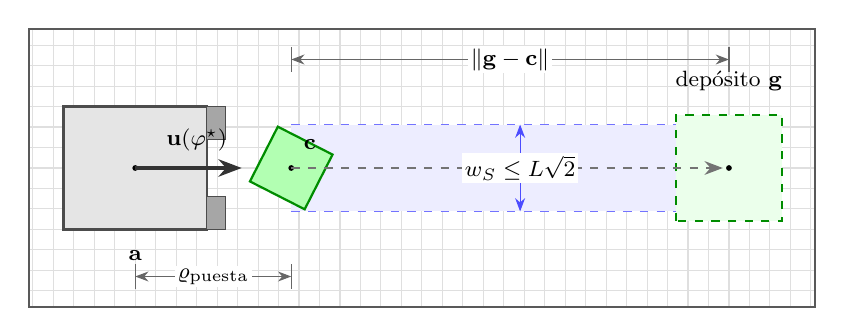
\begin{tikzpicture}[scale=0.52,>=Stealth,font=\small]
  \def\Lc{1.5}          % lado del cubo
  \def\Rw{3.0}          % ancho del rover
  \def\Rl{3.5}          % largo del rover
  \def\xa{0}            % x del centro del rover en la puesta
  \def\xc{3.81}         % x del centro del cubo  (rho_puesta = 152,4 mm)
  \def\xg{14.5}         % x del deposito

  % --- tablero
  \draw[gray!25,step=0.5] (-2.6,-3.4) grid (16.6,3.4);
  \draw[black!65,thick]   (-2.6,-3.4) rectangle (16.6,3.4);

  % --- corredor de empuje
  \fill[blue!7] (\xc,-1.061) rectangle (\xg,1.061);
  \draw[blue!55,dashed] (\xc, 1.061) -- (\xg, 1.061);
  \draw[blue!55,dashed] (\xc,-1.061) -- (\xg,-1.061);

  % --- deposito
  \draw[green!55!black,dashed,thick,fill=green!8]
       (\xg-1.3,-1.3) rectangle (\xg+1.3,1.3);
  \fill (\xg,0) circle (2pt);
  \node[font=\footnotesize,above=5pt] at (\xg,1.3) {depósito $\gv$};

  % --- cubo (inclinado theta)
  \begin{scope}[shift={(\xc,0)},rotate=-27]
    \draw[green!55!black,thick,fill=green!30]
         (-0.5*\Lc,-0.5*\Lc) rectangle (0.5*\Lc,0.5*\Lc);
  \end{scope}
  \fill (\xc,0) circle (2pt);
  \node[font=\footnotesize,above right=1pt and 1pt] at (\xc,0.15) {$\cc$};

  % --- rover en la pose de puesta
  \begin{scope}[shift={(\xa,0)}]
    \draw[black!70,thick,fill=black!10]
         (-0.5*\Rl,-0.5*\Rw) rectangle (0.5*\Rl,0.5*\Rw);
    \draw[black!70,fill=black!35] (0.5*\Rl,-0.5*\Rw)   rectangle (0.5*\Rl+0.45,-0.5*\Rw+0.8);
    \draw[black!70,fill=black!35] (0.5*\Rl, 0.5*\Rw-0.8) rectangle (0.5*\Rl+0.45, 0.5*\Rw);
    \fill (0,0) circle (2pt);
    \node[font=\footnotesize,below=4pt] at (0,-0.5*\Rw) {$\aaa$};
  \end{scope}

  % --- rumbo
  \draw[->,very thick,black!80] (\xa,0) -- (\xa+2.6,0);
  \node[font=\footnotesize,above=2pt] at (\xa+1.5,0.05) {$\uu(\varphi^\star)$};

  % --- eje de empuje
  \draw[->,thick,dashed,black!55] (\xc,0) -- (\xg-0.15,0);

  % --- cota de anchura del corredor
  \draw[<->,blue!70] (9.4,-1.061) -- (9.4,1.061);
  \node[font=\footnotesize,fill=white,inner sep=1pt] at (9.4,0) {$w_S \le L\sqrt2$};

  % --- cota rho_puesta
  \draw[black!60] (\xa,-2.35) -- (\xa,-2.95);
  \draw[black!60] (\xc,-2.35) -- (\xc,-2.95);
  \draw[<->,black!60] (\xa,-2.65) -- (\xc,-2.65);
  \node[font=\footnotesize,fill=white,inner sep=1pt] at (0.5*\xc,-2.65)
       {$\varrho_{\mathrm{puesta}}$};

  % --- cota recorrido de empuje
  \draw[black!60] (\xc,2.35) -- (\xc,2.95);
  \draw[black!60] (\xg,2.35) -- (\xg,2.95);
  \draw[<->,black!60] (\xc,2.65) -- (\xg,2.65);
  \node[font=\footnotesize,fill=white,inner sep=1pt] at (0.5*\xc+0.5*\xg,2.65)
       {$\|\gv-\cc\|$};
\end{tikzpicture}
\caption{Geometría de contacto y corredor de empuje (escala $1\ \mathrm{u} = 40\ \mathrm{mm}$).
El rover alcanza la pose de puesta $(\aaa,\varphi^\star)$, avanza según
$\uu(\varphi^\star)$ y empuja el cubo a lo largo del segmento $[\cc,\gv]$. El corredor
barrido (sombreado) tiene semiancho acotado por $L\sqrt2/2$ cualquiera sea la
inclinación $\theta$ del cubo, por el teorema \ref{teo:anchura}.}
\label{fig:contacto}
\end{figure}

\subsection{El embudo de tolerancia}
\label{sec:embudo}

Este es el resultado que decide si el sistema puede empujar sin conocer $\theta$.

\begin{teorema}[Embudo de tolerancia lateral]
\label{teo:embudo}
Sea el rover de ancho útil de paletas $W$ avanzando en la dirección $\uu(\varphi^\star)$
y sea $e$ el desplazamiento lateral entre el eje longitudinal del rover y el centro del
cubo, medido según $\uu_\perp(\varphi^\star)$. Una condición suficiente para que el cubo
quede íntegramente comprendido entre las paletas es
\begin{equation}
  |e| \;\le\; e_{\max}(\theta) \;=\; \frac{W - w_S(\varphi^\star)}{2}
   \;=\; \frac{W - L\big(|\cos\Delta| + |\sin\Delta|\big)}{2}.
  \label{eq:emax}
\end{equation}
Por el teorema \ref{teo:anchura}, para todo $\theta$:
\begin{equation}
  \boxed{\
  \frac{W - L\sqrt2}{2} \;\le\; e_{\max}(\theta) \;\le\; \frac{W - L}{2}.\ }
  \label{eq:emax-cota}
\end{equation}
Con el ancho \emph{útil del canal} $W = W_u = 93{,}50\ \mathrm{mm}$
(teorema \ref{teo:junta}) y $L = 60\ \mathrm{mm}$:
\[
  e_{\max} \in \big[\,4{,}32\ \mathrm{mm};\ 16{,}75\ \mathrm{mm}\,\big]
  \;=\; \big[\,0{,}216;\ 0{,}838\,\big]\ \text{celdas}.
\]
El ancho que entra aquí es $W_u$, no la huella $W_{\mathrm{ext}}$: lo que sujeta al cubo
son las caras interiores de los paneles (observación \ref{obs:dos-anchos}).
\end{teorema}

\begin{demo}
Proyectando sobre la dirección transversal $\uu_\perp(\varphi^\star)$: el rover ocupa el
intervalo $[-W/2, W/2]$ y el cubo, centrado en $e$, ocupa
$\big[e - \tfrac{w_S}{2},\ e + \tfrac{w_S}{2}\big]$ por la definición de anchura
proyectada. La inclusión del segundo intervalo en el primero equivale a
$e + \tfrac{w_S}{2}\le \tfrac{W}{2}$ y $e - \tfrac{w_S}{2} \ge -\tfrac{W}{2}$, es decir
$|e| \le (W-w_S)/2$. La cota \eqref{eq:emax-cota} se obtiene sustituyendo los extremos
de $w_S$ del teorema \ref{teo:anchura}, y la aplicación es monótona decreciente en
$w_S$, de modo que el mínimo de $e_{\max}$ corresponde al máximo de $w_S$.
\end{demo}

\begin{resultado}
\textbf{Corolario operativo: la factibilidad se conserva, pero el presupuesto de control
se vuelve negativo en una banda de orientaciones.} La cota inferior universal
$e_{\max} \ge (W_u - L\sqrt2)/2 = 4{,}32\ \mathrm{mm}$ se cumple para \emph{toda}
inclinación $\theta$: el cubo siempre \emph{entra} entre las paletas, porque
$L\sqrt2 = 84{,}85 < 93{,}50 = W_u$. La factibilidad geométrica está garantizada.

Lo que no está garantizado es poder aprovecharla. Descontando la incertidumbre de la
visión ($\sigma_{\mathrm{vis}} = 5\ \mathrm{mm}$), el presupuesto para el error de
control es
\[
  e^{\max}_{\mathrm{control}} \;=\; e_{\max} - \sigma_{\mathrm{vis}}
  \;=\;
  \begin{cases}
    4{,}32 - 5{,}00 \;=\; \mathbf{-0{,}68\ \mathrm{mm}}, & \Delta \equiv 45\grados,\\[3pt]
    16{,}75 - 5{,}00 \;=\; 11{,}75\ \mathrm{mm}, & \Delta \equiv 0\grados .
  \end{cases}
\]
El peor caso es \textbf{negativo}: la sola incertidumbre de la medición excede la
tolerancia disponible, aun con un controlador perfecto. Esto invierte la conclusión de
la versión anterior de este documento. Con $W = 120\ \mathrm{mm}$ (valor supuesto)
conocer $\theta$ era una mejora de eficiencia; con el cuerpo del chasis ($98{,}66$, sin
descontar la junta) pasaba a ser una
palanca de robustez; con el valor real $W_u = 93{,}50\ \mathrm{mm}$
\textbf{es un requisito}: existen orientaciones para las cuales el empuje ciego no tiene
margen alguno, y la proposición \ref{prop:ventana} las delimita.
\end{resultado}

\begin{proposicion}[Ventana angular admisible]
\label{prop:ventana}
Sea $\sigma_{\mathrm{vis}}$ la incertidumbre de la visión y $m\ge 0$ el margen de control
que se le quiera reservar al controlador. El conjunto de desalineaciones
$\Delta = \varphi^\star - \theta$ para las que el presupuesto
$e_{\max}(\Delta) - \sigma_{\mathrm{vis}} \ge m$ es no vacío es
\begin{equation}
  \mathcal V(m) \;=\; \left\{\, \Delta \ :\
  \big|\sin 2\Delta\big| \;\le\;
  \left(\frac{W_u - 2(\sigma_{\mathrm{vis}} + m)}{L}\right)^{\!2} - 1 \,\right\},
  \label{eq:ventana}
\end{equation}
un entorno de $\Delta \equiv 0 \pmod{90\grados}$, y es vacío si
$W_u < L + 2(\sigma_{\mathrm{vis}}+m)$.
\end{proposicion}

\begin{demo}
Por \eqref{eq:emax} y el teorema \ref{teo:anchura},
$e_{\max}(\Delta) = \big(W_u - L\sqrt{1+|\sin 2\Delta|}\big)/2$. Imponer
$e_{\max} - \sigma_{\mathrm{vis}} \ge m$ equivale a
$L\sqrt{1+|\sin2\Delta|} \le W_u - 2(\sigma_{\mathrm{vis}}+m)$; ambos miembros son no
negativos cuando el derecho lo es, y elevando al cuadrado se obtiene \eqref{eq:ventana}.
La condición de no vacuidad corresponde a $|\sin2\Delta| = 0$.
\end{demo}

\begin{resultado}
\textbf{Regla de apuntado.} Con $W_u = 93{,}50$, $L = 60$ y
$\sigma_{\mathrm{vis}} = 5\ \mathrm{mm}$:
\begin{center}
\begin{tabular}{lrr}
\toprule
Margen de control exigido $m$ & Ventana $|\Delta| \le$ & Fracción de orientaciones \\
\midrule
$0\ \mathrm{mm}$ (presupuesto nulo) & $34{,}76\grados$ & $77{,}2\%$ \\
$3\ \mathrm{mm}$ & $\mathbf{20{,}97\grados}$ & $\mathbf{46{,}6\%}$ \\
$5\ \mathrm{mm}$ & $12{,}86\grados$ & $28{,}6\%$ \\
$8\ \mathrm{mm}$ & --- & $0\%$ \\
\bottomrule
\end{tabular}
\end{center}
Complementariamente, la \textbf{banda de presupuesto negativo} es
\[
  \Delta \in (\,34{,}76\grados;\ 55{,}24\grados\,) \pmod{90\grados},
\]
el $22{,}8\%$ de las orientaciones. En ella no existe controlador, por perfecto que sea,
que garantice la captura con la incertidumbre de visión actual.

\smallskip
La regla operativa es en consecuencia: \textbf{apuntar el empuje a menos de
$\sim\!21\grados$ de la normal a una cara del cubo}. Como las caras se repiten cada
$90\grados$, hay cuatro direcciones admisibles y la restricción cuesta poco en
planificación --- pero exige conocer $\theta$.
\end{resultado}

\begin{observacion}[Sensibilidad al ancho útil: ya no es un parámetro libre]
\label{obs:medirW}
En una versión anterior de este documento, $W$ y $\Lambda$ se tomaban del cuerpo de rover
declarado en la configuración del generador sintético ($120 \times 140\ \mathrm{mm}$) y
se señalaban como el parámetro crítico a medir físicamente. \textbf{Ya no hace falta
medirlo:} los valores exactos están en el archivo de fabricación del repositorio, y son
otros (sección \ref{sec:dxf}).

La sensibilidad sigue siendo la que era,
\[
  \frac{\partial e_{\max}}{\partial W} = \frac{1}{2},
  \qquad
  e_{\max}^{\min}(W) = \frac{W - 84{,}853}{2}\ \mathrm{mm},
\]
y el umbral cualitativo también: el empuje deja de ser factible para \emph{toda}
inclinación cuando $W < L\sqrt2 = 84{,}853\ \mathrm{mm}$. El canal real mide
$93{,}50\ \mathrm{mm}$, de modo que queda por encima del umbral con
$8{,}65\ \mathrm{mm}$ de holgura --- contra los $13{,}81\ \mathrm{mm}$ que daba el cuerpo
del chasis sin descontar la junta, y los $35{,}15\ \mathrm{mm}$ del valor supuesto
original. La sucesión $35{,}15 \to 13{,}81 \to 8{,}65$ mide cuánto margen aparente
destruyó cada corrección de dato.
\end{observacion}

\begin{observacion}[Umbral angular en el régimen intermedio]
Si $L \le W < L\sqrt2$, la condición $w_S(\varphi^\star)\le W$ del
teorema \ref{teo:embudo} se escribe, con $\Delta = \varphi^\star-\theta$ y usando
$|\cos\Delta| + |\sin\Delta| = \sqrt{1+|\sin 2\Delta|}$, como
\begin{equation}
  \big|\sin 2\Delta\big| \;\le\; \left(\frac{W}{L}\right)^{\!2} - 1 .
  \label{eq:regimen}
\end{equation}
Con el ancho útil real, $(W_u/L)^2 - 1 = 1{,}428 > 1$: la desigualdad se cumple para
todo $\Delta$ y el régimen intermedio no se alcanza. El cubo entra siempre, cualquiera
sea su inclinación. Obsérvese, sin embargo, que \eqref{eq:regimen} es exactamente
\eqref{eq:ventana} con $\sigma_{\mathrm{vis}} = m = 0$: el régimen intermedio no se
alcanza para la \emph{entrada}, pero sí para el \emph{presupuesto de control}, que es la
condición que de verdad opera (proposición \ref{prop:ventana}).
\end{observacion}

\begin{observacion}[Rotación inducida por el empuje]
Si la línea de acción de la fuerza de empuje no pasa por el centro de fricción del cubo,
el empuje induce rotación. La condición geométrica de empuje sin giro es que el eje
longitudinal del rover contenga al centro $\cc$, es decir $e = 0$. Para $e \ne 0$ el
sentido de giro queda determinado por la regla clásica de votación de Mason entre la
línea de empuje y las dos aristas del cono de fricción respecto del centro de fricción;
su desarrollo pertenece a la mecánica del contacto y queda fuera del alcance de este
documento. La consecuencia \emph{geométrica} relevante es que $\theta$ evoluciona
durante el transporte, lo que refuerza el argumento del corolario anterior: cualquier
estimación de $\theta$ hecha antes del contacto se degrada durante el empuje, y por eso
la planificación debe apoyarse en cotas válidas para todo $\theta$.
\end{observacion}

\subsection{Corredor de empuje y factibilidad}

\begin{definicion}[Corredor de empuje]
El conjunto barrido por el cubo al ser empujado de $\cc$ a $\gv$ está contenido en el
rectángulo redondeado
\begin{equation}
  \mathcal K(\cc,\gv) \;=\; [\cc,\gv]\ \oplus\ D_{\varrho}, \qquad \varrho = \frac{L\sqrt2}{2},
  \label{eq:corredor}
\end{equation}
y el conjunto barrido por el rover está contenido en
$\mathcal K_{\mathrm{rov}} = [\aaa,\ \gv - \varrho_{\mathrm{cont}}\dd] \oplus D_{R_{\mathrm{rov}}}$.
\end{definicion}

\begin{proposicion}[Condición de factibilidad del empuje directo]
\label{prop:factible}
El empuje directo de $\cc$ a $\gv$ es geométricamente factible si y solo si se cumplen
simultáneamente:
\begin{enumerate}[label=(F\arabic*),leftmargin=3em,itemsep=2pt]
\item \textbf{Punto de puesta admisible:} $\aaa \in \mathcal C_{\mathrm{libre}}$, con
      $\aaa$ dado por \eqref{eq:puesta};
\item \textbf{Corredor libre:} $\mathcal K(\cc,\gv) \cap \big(\bigcup_j O_j\big) = \emptyset$,
      donde los $O_j$ incluyen los otros cubos y el otro rover;
\item \textbf{Corredor del rover libre:} $\mathcal K_{\mathrm{rov}} \subset \mathcal C_{\mathrm{libre}}$;
\item \textbf{Contención de frontera:} $\mathcal K(\cc,\gv) \subset \Omega^{\oplus 3{,}5}$,
      donde el inflado de $3{,}5$ celdas reconoce el borde muerto del tablero físico.
\end{enumerate}
\end{proposicion}

\begin{observacion}[Sobre F1 en los depósitos de esquina]
Los depósitos están en las tres esquinas que no son la de salida:
$(40{,}5;\,2{,}5)$, $(2{,}5;\,40{,}5)$ y $(40{,}5;\,40{,}5)$ celdas. Al final del empuje
el rover está en $\gv - \varrho_{\mathrm{cont}}\dd$, es decir \emph{hacia adentro} de la
cancha respecto del depósito, a unas $5{,}6$ celdas. Como $\gv$ dista al menos
$2{,}5$ celdas de la frontera $\Omega$ y el tablero físico ofrece $3{,}5$ celdas
adicionales, la condición F1 se satisface para todo depósito. La restricción activa no
es la frontera sino el punto de puesta \emph{inicial}, que exige
$\cc - \varrho_{\mathrm{puesta}}\dd \in \mathcal C_{\mathrm{libre}}$: si el cubo está
pegado al borde opuesto al depósito, el rover no cabe detrás.
\end{observacion}

\begin{corolario}[Zona de puesta inviable]
Un cubo en posición $\cc$ no admite empuje directo hacia $\gv$ si
\begin{equation}
  \cc - \varrho_{\mathrm{puesta}}\,\dd \notin \Omega^{\oplus 3{,}5},
\end{equation}
es decir si $\cc$ pertenece a la banda de espesor $\varrho_{\mathrm{puesta}}$ adyacente a
la frontera del lado opuesto al depósito. En ese caso se requiere la descomposición
multi-tramo de la sección \ref{sec:multitramo}.
\end{corolario}

\subsection{La ruta canónica y su funcional de costo}

\begin{definicion}[Ruta de tres fases]
La ruta canónica de transporte de un cubo consta de:
\begin{description}[leftmargin=2.6em,style=nextline,font=\normalfont\itshape]
\item[Fase A --- aproximación.] De la pose actual $(\pp_0,\theta_0)$ a la pose de puesta
      $(\aaa, \varphi^\star)$, sin tocar el cubo.
\item[Fase B --- empuje.] Traslación rectilínea a lo largo de $\dd$ desde $\aaa$ hasta
      $\gv - \varrho_{\mathrm{cont}}\dd$, manteniendo el rumbo $\varphi^\star$.
\item[Fase C --- retirada.] Retroceso una distancia $r$ a lo largo de $-\dd$ para
      liberar el cubo antes de la siguiente tarea.
\end{description}
\end{definicion}

\begin{teorema}[Costo de la fase A bajo locomoción diferencial]
\label{teo:RTR}
Un rover de locomoción diferencial puede girar en el lugar. Restringiendo la clase de
maniobras a \emph{giro--traslación--giro} (\textsc{gtg}), y suponiendo velocidad lineal
máxima $v$ y velocidad angular máxima $\omega$, el costo temporal mínimo de la fase A es
\begin{equation}
  T_A \;=\; \min\Big\{\,T^{+},\ T^{-}\,\Big\},
  \label{eq:TA}
\end{equation}
con
\begin{align}
  T^{+} &= \frac{\big|\delta(\varphi_{0},\theta_0)\big|}{\omega}
         + \frac{\|\aaa - \pp_0\|}{v}
         + \frac{\big|\delta(\varphi^\star, \varphi_{0})\big|}{\omega},
  \label{eq:Tplus}\\
  T^{-} &= \frac{\big|\delta(\varphi_{0}+180\grados,\ \theta_0)\big|}{\omega}
         + \frac{\|\aaa - \pp_0\|}{v}
         + \frac{\big|\delta(\varphi^\star,\ \varphi_{0}+180\grados)\big|}{\omega},
  \label{eq:Tminus}
\end{align}
donde $\varphi_{0} = \atantwo\big(-(a_y - p_{0,y}),\ a_x - p_{0,x}\big)$ es el rumbo del
segmento $\pp_0 \to \aaa$, y $\delta$ es la diferencia angular \eqref{eq:delta}.
\end{teorema}

\begin{demo}
Dentro de la clase \textsc{gtg}, la trayectoria queda determinada por el rumbo de
traslación $\psi$: el rover gira de $\theta_0$ a $\psi$, traslada, y gira de $\psi$ a
$\varphi^\star$. Para que la traslación lleve el centro de $\pp_0$ a $\aaa$ en línea
recta hay solo dos opciones: avanzar con $\psi = \varphi_0$, o retroceder con
$\psi = \varphi_0 + 180\grados$. La longitud recorrida es $\|\aaa-\pp_0\|$ en ambos
casos. Los tiempos de giro son proporcionales a la magnitud angular mínima, que es
$|\delta(\cdot,\cdot)|$ por definición de \eqref{eq:delta}. Tomando el mínimo entre las
dos opciones se obtiene \eqref{eq:TA}.
\end{demo}

\begin{corolario}[Regla exacta de decisión avance/retroceso]
\label{cor:retroceso}
Escribiendo $A = |\delta(\varphi_0,\theta_0)|$ (giro inicial) y
$B = |\delta(\varphi^\star,\varphi_0)|$ (giro final), y usando la identidad
$|\delta(\varphi_0+180\grados,\,x)| = 180\grados - |\delta(\varphi_0,x)|$, la diferencia
de costos de \eqref{eq:Tplus} y \eqref{eq:Tminus} es
\begin{equation}
  T^{+} - T^{-} \;=\; \frac{2\,\big(A + B - 180\grados\big)}{\omega} .
  \label{eq:regla-retroceso}
\end{equation}
Por lo tanto \textbf{conviene retroceder si y solo si $A + B > 180\grados$}.
\end{corolario}

\begin{demo}
Sustituyendo la identidad en \eqref{eq:Tminus}, el término de traslación se cancela y
queda
$T^{-} = \big[(180\grados - A) + (180\grados - B)\big]/\omega + \|\aaa-\pp_0\|/v$.
Restando de \eqref{eq:Tplus} se obtiene \eqref{eq:regla-retroceso}. La identidad se
verifica notando que $\delta(\varphi_0+180\grados,x)$ y $\delta(\varphi_0,x)$ tienen
signos opuestos y magnitudes que suman $180\grados$, por ser $\varphi_0$ y
$\varphi_0+180\grados$ antipodales.
\end{demo}

\begin{observacion}[La regla ingenua no sirve]
Es tentador decidir mirando solo el primer giro: «retroceder si $A > 90\grados$». Esa
regla \textbf{acierta apenas el $75\%$} de las veces sobre ternas
$(\pp_0,\theta_0,\aaa,\varphi^\star)$ uniformes, porque ignora que el retroceso también
cambia el giro \emph{final}. El error se manifiesta como maniobras con un giro de más,
síntoma que suele atribuirse al controlador de bajo nivel.
\end{observacion}

\begin{observacion}[Sobre la optimalidad]
$T_A$ es óptimo \emph{dentro de la clase} \textsc{gtg}. La trayectoria de tiempo mínimo
sin esa restricción, para un vehículo diferencial con velocidades acotadas, pertenece a
la familia de Balkcom--Mason y puede ser estrictamente más rápida al superponer giro y
traslación. Se adopta \textsc{gtg} porque desacopla completamente los grados de libertad
---lo que simplifica el control y la verificación--- y porque su costo acota
superiormente al óptimo, sirviendo así como cota conservadora para comparar rutas.
\end{observacion}

\begin{definicion}[Costo total de una tarea de transporte]
\begin{equation}
  \mathcal J(\pp_0,\theta_0;\ \cc,\gv)
  \;=\; \underbrace{T_A}_{\text{aproximación}}
  \;+\; \underbrace{\frac{\|\gv-\cc\| + \varrho_{\mathrm{puesta}} - \varrho_{\mathrm{cont}}}{v_{\mathrm{emp}}}}_{\text{empuje}}
  \;+\; \underbrace{\frac{r}{v}}_{\text{retirada}} ,
  \label{eq:costo}
\end{equation}
donde $v_{\mathrm{emp}} < v$ es la velocidad de empuje, reducida respecto de la de
traslación libre por la carga y por la necesidad de corrección continua.
\end{definicion}

\subsection{Selección del lado de aproximación}

El punto de puesta \eqref{eq:puesta} está determinado por $\dd$, pero llegar a él puede
requerir rodear el cubo. Se formaliza el costo de ese rodeo.

\begin{definicion}[Anillo de aproximación]
El lugar geométrico de posiciones desde las que el rover puede tocar el cubo sin
colisionar con él es la circunferencia
\begin{equation}
  \mathcal A(\cc) \;=\; \big\{\, \cc + \varrho_{\mathrm{puesta}}\,\uu(\psi) \ :\ \psi \in [0\grados,360\grados) \,\big\}.
\end{equation}
El punto de puesta correcto es $\aaa = \cc + \varrho_{\mathrm{puesta}}\,\uu(\varphi^\star + 180\grados)$,
es decir el punto del anillo diametralmente opuesto al depósito.
\end{definicion}

\begin{proposicion}[Costo de reposicionamiento sobre el anillo]
\label{prop:anillo}
Si el rover se encuentra sobre el anillo en el ángulo $\psi_0$ y debe alcanzar
$\psi^\star = \varphi^\star + 180\grados$, el desplazamiento a lo largo del anillo tiene
longitud
\begin{equation}
  \ell_{\mathrm{arco}} \;=\; \varrho_{\mathrm{puesta}}\cdot \frac{\pi}{180\grados}\cdot \rho_{360}(\psi^\star, \psi_0),
  \label{eq:arco}
\end{equation}
y este recorrido es libre de colisión con el cubo por construcción. Aproximar el arco
por una cuerda recta reduce la distancia pero puede violar la restricción de no
colisión si $\rho_{360}(\psi^\star,\psi_0) > 2\arccos\!\big(\varrho_{\mathrm{cont}}/\varrho_{\mathrm{puesta}}\big)$.
\end{proposicion}

\begin{demo}
La longitud de un arco de circunferencia de radio $\varrho$ y ángulo $\Delta\psi$ en
radianes es $\varrho\,\Delta\psi$; \eqref{eq:arco} es la conversión de grados a
radianes con $\Delta\psi$ mínimo, dado por $\rho_{360}$. Para la segunda afirmación: la
cuerda que subtiende un ángulo $2\alpha$ en una circunferencia de radio
$\varrho_{\mathrm{puesta}}$ dista $\varrho_{\mathrm{puesta}}\cos\alpha$ del centro; la
condición de no penetrar el disco de contacto es
$\varrho_{\mathrm{puesta}}\cos\alpha \ge \varrho_{\mathrm{cont}}$, es decir
$2\alpha \le 2\arccos(\varrho_{\mathrm{cont}}/\varrho_{\mathrm{puesta}})$.
\end{demo}

\begin{resultado}
\textbf{Regla práctica.} Con $\varrho_{\mathrm{puesta}} = 129{,}43\ \mathrm{mm}$
(tomando $s = 40\ \mathrm{mm}$) y $\varrho_{\mathrm{cont}} = 89{,}43\ \mathrm{mm}$:
\[
  2\arccos\!\left(\frac{89{,}43}{129{,}43}\right) \;=\; 92{,}59\grados .
\]
Es decir: reposicionamientos de hasta $92{,}59\grados$ alrededor del cubo pueden hacerse
en línea recta; más allá de ese umbral hay que recorrer el arco o insertar un punto
intermedio.
\end{resultado}

\subsection{Rutas con obstáculos: grafo de visibilidad}

\begin{teorema}[Estructura de la ruta más corta entre discos]
\label{teo:visibilidad}
Sea $\mathcal C_{\mathrm{libre}}$ el complemento de una unión finita de discos abiertos
disjuntos $\{D_j\}$ dentro de un rectángulo. La ruta más corta entre dos puntos de
$\mathcal C_{\mathrm{libre}}$ existe y está compuesta exclusivamente por:
\begin{enumerate}[label=(\alph*),leftmargin=2.2em]
\item segmentos rectos tangentes a los discos (o que unen los extremos con tangencias), y
\item arcos de circunferencia sobre las fronteras $\partial D_j$.
\end{enumerate}
\end{teorema}

\begin{demo}[Esbozo]
La existencia sigue del teorema de Arzelà--Ascoli aplicado a la familia de caminos de
longitud acotada en un compacto. Para la estructura: en todo subintervalo cuyo interior
no toca ningún $\partial D_j$, la ruta minimiza longitud en un abierto del plano, luego
es un segmento recto. En un subintervalo contenido en algún $\partial D_j$, la ruta debe
seguir la geodésica de esa curva, que es el propio arco. En los puntos de transición, la
condición de primer orden de minimalidad impone tangencia; de lo contrario existiría una
variación que acorta la ruta.
\end{demo}

\begin{corolario}[Discretización]
El problema continuo se reduce a un problema de grafo: los nodos son el origen, el
destino y los puntos de tangencia; las aristas son los segmentos tangentes y los arcos
libres, ponderados por su longitud. La ruta óptima se obtiene con Dijkstra sobre ese
grafo, cuyo tamaño es $O(n^2)$ para $n$ discos. En esta edición del reto la lista de
obstáculos llega vacía, de modo que $n \le 3$: los otros dos cubos y el otro rover.
\end{corolario}

\subsection{Empuje multi-tramo}
\label{sec:multitramo}

\begin{definicion}[Descomposición en tramos]
Cuando el empuje directo no es factible (proposición \ref{prop:factible}), se busca una
poligonal $\cc = \mathbf z_0 \to \mathbf z_1 \to \cdots \to \mathbf z_M = \gv$ tal que
cada tramo $[\mathbf z_{i-1}, \mathbf z_i]$ sea individualmente factible. El costo total
es
\begin{equation}
  \mathcal J_{\mathrm{multi}}
  \;=\; \sum_{i=1}^{M} \frac{\|\mathbf z_i - \mathbf z_{i-1}\|}{v_{\mathrm{emp}}}
  \;+\; \sum_{i=1}^{M-1} \Big(\underbrace{\tfrac{r}{v}}_{\text{retirada}}
  + \underbrace{\tfrac{\ell_{\mathrm{arco}}(\Delta\psi_i)}{v}}_{\text{reposicionamiento}}
  + \underbrace{\tfrac{\rho_{360}(\psi_{i+1},\psi_i)}{\omega}}_{\text{reorientación}}\Big),
  \label{eq:multitramo}
\end{equation}
donde $\Delta\psi_i$ es el cambio de dirección de empuje en el vértice $\mathbf z_i$ y
$\ell_{\mathrm{arco}}$ está dado por \eqref{eq:arco}.
\end{definicion}

\begin{observacion}[El costo de doblar]
El segundo sumatorio de \eqref{eq:multitramo} es el precio de cada quiebre de la
trayectoria del cubo: obliga a retirarse, rodear el cubo por el anillo y reorientarse.
Con los valores de la sección \ref{sec:parametros}, un quiebre de $90\grados$ cuesta del
orden de
\[
  \underbrace{\frac{r}{v}}_{40\ \mathrm{mm}/v}
  \;+\; \underbrace{\frac{\varrho_{\mathrm{puesta}}\,\pi/2}{v}}_{203{,}3\ \mathrm{mm}/v}
  \;+\; \frac{90\grados}{\omega}
  \;=\; \frac{243{,}3\ \mathrm{mm}}{v} + \frac{90\grados}{\omega},
\]
que es comparable a empujar $243\ \mathrm{mm}$ en línea recta. \emph{Conclusión de
diseño:} conviene fuertemente minimizar el número de quiebres antes que la longitud
total. Una poligonal de dos tramos rara vez compensa a una de un tramo aunque sea más
corta en distancia.
\end{observacion}

\subsection{Conjunto alcanzable bajo oclusión}
\label{sec:alcanzable}

\begin{definicion}[Conjunto alcanzable condicional]
Sea un cubo con última posición conocida $\cc_{\mathrm{obs}}$ y edad $\alpha$
(ecuación \eqref{eq:edad}). Bajo la hipótesis de que un cubo solo se mueve si un rover lo
empuja, el conjunto de posiciones posibles es
\begin{equation}
  \mathcal D(\alpha) \;=\;
  \begin{cases}
    \{\cc_{\mathrm{obs}}\}, & \text{si ningún rover pudo alcanzarlo en } \alpha, \\[6pt]
    \cc_{\mathrm{obs}} \oplus D_{v_{\mathrm{emp}}\,\alpha}, & \text{en caso contrario.}
  \end{cases}
  \label{eq:alcanzable}
\end{equation}
La condición del primer caso es
\begin{equation}
  \min_{j}\ \Big(\|\pp_j - \cc_{\mathrm{obs}}\| - \varrho_{\mathrm{cont}}\Big) \;>\; v\,\alpha ,
  \label{eq:no-alcanzable}
\end{equation}
donde $\pp_j$ recorre las posiciones conocidas de los rovers en el instante de la última
observación.
\end{definicion}

\begin{observacion}
Esta formulación es sensiblemente más informativa que inflar el radio de incertidumbre
proporcionalmente a $\alpha$ sin condicionar: un cubo lejos de ambos rovers y no visto
durante $3\ \mathrm{s}$ sigue estando \emph{exactamente} donde dice el último dato, porque
nada pudo moverlo. La oclusión más frecuente ---un rover encima del cubo--- es
precisamente el caso en que \eqref{eq:no-alcanzable} falla, y ahí la incertidumbre sí
crece; pero entonces el rover que ocluye es el propio, y su odometría cubre el hueco.
Que $\alpha$ sea alto no significa que el cubo se haya movido: significa que la visión no
lo ve.
\end{observacion}

\subsection{Restricciones de interfaz hacia las capas no cubiertas}

Las siguientes condiciones son consecuencias geométricas que las capas de control y
fusión sensorial ---fuera del alcance de este documento--- deben satisfacer:

\begin{enumerate}[label=RI\arabic*.,leftmargin=3em,itemsep=3pt]
\item \textbf{Error lateral acotado.} Durante la fase B, el controlador debe mantener
      \[
        |e| \;\le\; e_{\max} - \sigma_{\mathrm{vis}}
        \;=\;
        \begin{cases}
          4{,}32 - 5{,}00 = \mathbf{-0{,}68}\ \mathrm{mm}, & \Delta \equiv 45\grados \ \text{(peor caso)},\\[3pt]
          16{,}75 - 5{,}00 = 11{,}75\ \mathrm{mm}, & \Delta \equiv 0\grados \ \text{(cubo alineado)}.
        \end{cases}
      \]
      Con paletas paralelas esta cota es \emph{exacta}, no conservadora
      (proposición \ref{prop:canal}): no hay boca ancha que ayude a la captura. En el
      peor caso el requisito es \textbf{insatisfacible}, y por eso RI1 no puede
      formularse sola: exige acompañarse de RI2.
\item \textbf{Alineación angular del empuje (nueva, y ahora obligatoria).} El empuje debe
      apuntarse dentro de la ventana de la proposición \ref{prop:ventana}. Con un margen
      de control de $3\ \mathrm{mm}$:
      \[
        \boxed{\ \big|\,\varphi^\star - \theta\,\big| \;\le\; 21\grados \pmod{90\grados}.\ }
      \]
      Fuera de esa ventana el presupuesto lateral es inferior a $3\ \mathrm{mm}$, y en la
      banda $\Delta \in (34{,}76\grados;\ 55{,}24\grados)$ es directamente negativo. Esta
      restricción \textbf{no se puede satisfacer sin estimar $\theta$}: es el punto en el
      que la estimación de la inclinación deja de ser una optimización y pasa a ser
      condición de funcionamiento.
\item \textbf{Precisión angular de puesta.} El error de rumbo $\epsilon_\theta$ en la
      pose de puesta genera un error lateral
      $\|\aaa-\cc\|\sin\epsilon_\theta$ al alcanzar el cubo. Con
      $\|\aaa-\cc\| = \varrho_{\mathrm{puesta}} = 129{,}43\ \mathrm{mm}$ y el empuje ya
      alineado según RI2:
      \[
        \epsilon_\theta \;\le\; \arcsin\!\left(\frac{11{,}75}{129{,}43}\right) = 5{,}21\grados
        \quad (\Delta \equiv 0),
        \qquad
        \epsilon_\theta \;\le\; \arcsin\!\left(\frac{5{,}01}{129{,}43}\right) = 2{,}22\grados
        \quad (|\Delta| = 15\grados).
      \]
      \textbf{Este es el número que más pesa de todo el documento.} Sin alinear, el
      requisito no existe ---no hay $\epsilon_\theta$ admisible en el peor caso---; con
      el empuje alineado a una cara, exigir $5\grados$ de precisión de rumbo a un rover
      diferencial con giróscopo es razonable. La diferencia entre \emph{imposible} y
      \emph{razonable} es \emph{únicamente} conocer la inclinación del cubo.
\item \textbf{Frecuencia de corrección.} Con telemetría a $20\ \mathrm{Hz}$, el intervalo
      entre correcciones es $50\ \mathrm{ms}$. A velocidad de empuje $v_{\mathrm{emp}}$,
      la deriva lateral acumulada entre correcciones debe ser inferior al margen de RI1.
\item \textbf{Corte por latencia.} Si $\lambda > 500\ \mathrm{ms}$, el rover debe
      detenerse: geométricamente, la posición del cubo deja de estar acotada por
      \eqref{eq:alcanzable} con $\alpha$ pequeño y la garantía del embudo se pierde.
\end{enumerate}

% ================================================================ 5b
\section{Verificación sobre el rover físico}
\label{sec:medicion}

Las secciones anteriores derivan la geometría del archivo de fabricación. Esta la
contrasta contra el robot armado. Las mediciones se hicieron con regla escolar sin
calibrar, sobre una \textbf{versión preliminar} del rover, de modo que se tratan como
$\pm 1\ \mathrm{mm}$ y ninguna conclusión se apoya en un solo número.

\subsection{Cómo se mide con regla lo que parece necesitar calibrador}

El valor en disputa es $W_u$, y el umbral que decide es $94{,}85\ \mathrm{mm}$
---el ancho para el cual el presupuesto de control a $45\grados$ se anula---. Separar
$93{,}5$ de $94{,}9$ sobre un tramo de $94\ \mathrm{mm}$ excede la resolución del
instrumento. Pero la misma diferencia, leída sobre un \emph{hueco}, cae en el rango donde
la regla sí resuelve:

\begin{proposicion}[Medición del embudo por diferencia de huecos]
\label{prop:huecos}
Sea $h(\Delta)$ el hueco que queda entre el cubo y una paleta cuando el cubo, girado
$\Delta$, se apoya contra la otra. Entonces
\begin{equation}
  h(\Delta) \;=\; W_u - w_S(\Delta) \;=\; 2\,e_{\max}(\Delta),
  \label{eq:hueco}
\end{equation}
y en particular
\begin{equation}
  h(45\grados) - h(0\grados) \;=\; -L(\sqrt2 - 1),
  \label{eq:control-huecos}
\end{equation}
que \textbf{no depende de $W_u$}: es una identidad que solo involucra la arista del cubo,
y sirve como control de la propia medición.
\end{proposicion}

\begin{demo}
Por definición de anchura proyectada, el cubo ocupa un intervalo de longitud
$w_S(\Delta)$ en la dirección transversal; apoyado contra una paleta, el resto de la
sección, $W_u - w_S$, es el hueco. La segunda igualdad es \eqref{eq:emax}. Restando las
dos evaluaciones se cancela $W_u$ y queda $w_S(0)-w_S(45\grados) = L - L\sqrt2$.
\end{demo}

\subsection{Lo medido}

\begin{table}[htbp]
\centering
\small
\caption{Mediciones sobre el rover armado, y lo que el modelo predecía.}
\begin{tabular}{clrrl}
\toprule
\# & Magnitud & predicho & medido & lectura \\
\midrule
M1  & Hueco con cubo a $45\grados$ & $8{,}65$ & $9{-}10$ & $W_u = 94{,}35$ \\
M2  & Hueco con cubo alineado & $33{,}50$ & $33$ & $W_u = 93{,}00$ \\
M9  & Canal, medido directo & $93{,}50$ & $95$ & $W_u = 95{,}00$ \\
\midrule
M6  & Alcance de paletas $\lambda$ & --- & $\mathbf{55}$ & nuevo \\
M7  & Ancho máximo real & $99{,}50$ & $100$ & concuerda \\
M8  & Largo máximo real & $149$ & $150$ & concuerda \\
M10 & Paletas: piso a borde superior & --- & $0$ a $14$ & nuevo \\
M12 & Aristas del cubo & vivas & vivas & concuerda \\
M13 & Rueda: diámetro / trocha & --- & $33$ / $89$ & nuevo \\
\bottomrule
\end{tabular}
\end{table}

\begin{resultado}
\textbf{El control de \eqref{eq:control-huecos} se cumple.} La resta medida es
$33 - 9{,}5 = 23{,}5\ \mathrm{mm}$ contra los $L(\sqrt2-1) = 24{,}85$ que predice la
identidad: un desvío de $1{,}35\ \mathrm{mm}$, compatible con dos lecturas de regla. Las
mediciones son internamente coherentes y se pueden usar.
\end{resultado}

\begin{resultado}
\textbf{$W_u$ queda determinado dentro de un milímetro, y el presupuesto sigue siendo
nulo.} Las tres estimaciones ---$94{,}35$, $93{,}00$ y $95{,}00$--- promedian
$94{,}05 \pm 0{,}54\ \mathrm{mm}$. El valor deducido del archivo de fabricación,
$93{,}50$, cae a $1{,}0\sigma$: la medición \textbf{no lo refuta}.

Lo que importa no es el valor sino su consecuencia, y esa es robusta al error:
\[
  e^{\max}_{\mathrm{control}}(45\grados) \;=\; \frac{W_u - L\sqrt2}{2} - \sigma_{\mathrm{vis}}
  \;\in\; [\,-0{,}94;\ +0{,}13\,]\ \mathrm{mm}
\]
para todo $W_u$ en el intervalo de $\pm2\sigma$. \textbf{El presupuesto lateral es cero
dentro del error de medición, cualquiera sea el valor que se tome.} El teorema
\ref{teo:embudo} y la proposición \ref{prop:ventana} quedan confirmados sin necesidad de
un instrumento mejor.
\end{resultado}

\subsection{Lo que la medición sí refutó}

\begin{teorema}[El envolvente del rover estaba subestimado]
\label{teo:envolvente}
Sea $\lambda$ el alcance de las paletas por delante de la placa frontal. La huella del
rover \textbf{no es simétrica} respecto del centro del chasis: se extiende $\Lambda/2$
hacia atrás y $\Lambda/2 + \lambda$ hacia adelante. El disco envolvente centrado en el
chasis tiene radio
\begin{equation}
  R_{\mathrm{rov}} \;=\; \sqrt{\Big(\frac{\Lambda}{2}+\lambda\Big)^{2} + \Big(\frac{W_{\mathrm{ext}}}{2}\Big)^{2}},
  \label{eq:Rrov-real}
\end{equation}
y no $\tfrac12\sqrt{W_{\mathrm{ext}}^2+\Lambda^2}$ como se usó hasta aquí.
\end{teorema}

\begin{demo}
Inmediata: el punto más lejano del centro es la esquina exterior de una punta de paleta,
en $(\Lambda/2+\lambda,\ \pm W_{\mathrm{ext}}/2)$.
\end{demo}

\begin{resultado}
\textbf{Hallazgo H-12.} Con $\lambda = 55\ \mathrm{mm}$ medido,
\[
  R_{\mathrm{rov}} = 113{,}49\ \mathrm{mm} \quad\text{contra los}\quad 68{,}44\ \mathrm{mm}
  \quad\text{que usaba el modelo: una subestimación del } \mathbf{66\%}.
\]
Es un error \emph{del lado peligroso}: el planificador creía pasar por huecos por los que
no pasa. Tres consecuencias, en orden de gravedad:
\begin{enumerate}[label=(\alph*),leftmargin=2.2em,itemsep=3pt]
\item \textbf{El anillo de aproximación deja de librar el cubo.} Rodear el cubo a
      $\varrho_{\mathrm{puesta}} = 129{,}43\ \mathrm{mm}$ lo \emph{barre} con las paletas.
      Girar detrás del cubo exige
      \[
        \varrho_{\mathrm{man}} \;=\; R_{\mathrm{rov}} + \frac{L\sqrt2}{2} \;=\; 155{,}9\ \mathrm{mm},
      \]
      y el acceso pasa a ser en dos tramos: al anillo de maniobra primero, y desde ahí en
      línea recta por el propio eje de empuje.
\item \textbf{La zona trampa crece.} Con $\varrho_{\mathrm{man}}$ en lugar de
      $\varrho_{\mathrm{puesta}}$, la fracción de cancha desde la que un cubo no puede
      alejarse de un borde sube de $5{,}03\%$ a $6{,}46\%$, y la banda junto a la pared de
      $2{,}97$ a $4{,}55$ celdas. Los depósitos están a $2{,}5$ celdas del borde: quedan
      \emph{dentro} de esa banda.
\item \textbf{$\varrho_{\mathrm{cont}}$ no cambia.} Como $\lambda = 55 > L\sqrt2/2 = 42{,}43$,
      el cubo entra en el canal hasta tocar la placa frontal, que es la que empuja. La
      distancia de contacto sigue siendo $89{,}43\ \mathrm{mm}$.
\end{enumerate}
\end{resultado}

\begin{proposicion}[Tramo de contención previo al contacto]
\label{prop:tramo}
Entre el instante en que las puntas de las paletas alcanzan al cubo y el instante del
contacto con la placa frontal, el rover avanza exactamente $\lambda$, con independencia de
la orientación del cubo.
\end{proposicion}

\begin{demo}
Sea $x$ la posición de la placa sobre el eje de empuje; las puntas están en $x+\lambda$ y
la cara trasera del cubo en $c - w_S/2$. Las puntas alcanzan al cubo cuando
$x+\lambda = c - w_S/2$ y la placa lo toca cuando $x = c - w_S/2$. La diferencia es
$\lambda$, y $w_S$ se cancela.
\end{demo}

\begin{observacion}[La contención es parcial]
Como $\lambda = 55 < L = 60 \le w_S$, el cubo \emph{siempre} sobresale por delante de las
puntas. Las paletas cubren entre el $92\%$ de su extensión con el cubo alineado y el
$65\%$ a $45\grados$: la contención es más débil justo en la orientación de peor
tolerancia. Sumado a la proposición \ref{prop:canal}, que dice que el canal contiene pero
no centra, el resultado operativo es que \textbf{la alineación tiene que estar lograda
antes de que las puntas alcancen el cubo}, y el sistema no dispone de ningún mecanismo
para corregirla después.
\end{observacion}

\subsection{Lo que la medición confirmó y el modelo no sabía}

\begin{enumerate}[label=(\alph*),leftmargin=2.2em,itemsep=4pt]
\item \textbf{El polígono de apoyo es el que supuso el modelo del precipicio.} Las paletas
      llegan al piso sin separación medible, de modo que el apoyo son las dos ruedas más
      las puntas de los brazos, exactamente como se postuló en la sección
      \ref{sec:precipicio} sin evidencia. La consecuencia práctica es que \textbf{una
      paleta en voladizo sobre el vacío no vuelca al rover}: solo pierde ese apoyo, y las
      ruedas lo sostienen. Por eso la restricción de frontera se evalúa sobre el chasis y
      no sobre la huella completa.
\item \textbf{No hay riesgo de vuelco del cubo.} Las paletas abarcan de $0$ a
      $14\ \mathrm{mm}$ sobre el piso, así que el empuje actúa a unos $7\ \mathrm{mm}$ de
      altura, muy por debajo de la mitad del cubo ($30\ \mathrm{mm}$). La hipótesis H6
      ---contacto plano, el cubo no vuelca--- queda respaldada.
\item \textbf{Las ruedas no sobresalen.} Trocha $89\ \mathrm{mm}$ contra un canal de
      $\sim\!94$: quedan dentro de la huella de acrílico, lo que valida usar
      $W_{\mathrm{ext}}$ como ancho de colisión.
\item \textbf{Constantes de odometría.} Rueda de $33\ \mathrm{mm}$ de diámetro: una vuelta
      son $103{,}67\ \mathrm{mm}$ de avance. Trocha de $89\ \mathrm{mm}$: un giro de
      $90\grados$ en el lugar son $69{,}90\ \mathrm{mm}$ por rueda. Son los dos números que
      convierten pulsos de encoder en milímetros y grados, y sin ellos la odometría que
      debe cubrir los huecos de oclusión no se puede calibrar.
\end{enumerate}

% ================================================================ 6
\section{Cuadro maestro de parámetros}
\label{sec:parametros}

\begin{table}[htbp]
\centering
\small
\caption{Parámetros del modelo. Origen: R = repositorio (archivo indicado);
D = derivado en este documento; M = medido sobre el rover armado (regla, $\pm1\ \mathrm{mm}$).}
\begin{tabular}{llllp{4.2cm}}
\toprule
Símbolo & Descripción & Valor & Or. & Fuente / derivación \\
\midrule
\multicolumn{5}{l}{\textit{Cancha}}\\
$C\times F$ & Cancha efectiva & $43\times43$ celdas & R & \texttt{config\_vision.json} \\
$\xi$ & Lado de celda & $20{,}0\ \mathrm{mm}$ & R & \texttt{config\_vision.json} \\
--- & Cancha en métrico & $860\times860\ \mathrm{mm}$ & D & $43\cdot20$ \\
--- & Tablero físico & $50\times50$ cuadros & R & \texttt{config\_vision.json} \\
--- & Borde muerto & $3{,}5$ celdas/lado & D & $(50-43)/2$ \\
$\pp_{\mathrm{start}}$ & Esquina de salida & $(2{,}5;\,2{,}5)$ & R & \texttt{config\_vision.json} \\
$\gg_{\mathrm{verde}}$ & Depósito verde & $(40{,}5;\,2{,}5)$ & R & \texttt{config\_vision.json} \\
$\gg_{\mathrm{azul}}$ & Depósito azul & $(2{,}5;\,40{,}5)$ & R & \texttt{config\_vision.json} \\
$\gg_{\mathrm{rojo}}$ & Depósito rojo & $(40{,}5;\,40{,}5)$ & R & \texttt{config\_vision.json} \\
\midrule
\multicolumn{5}{l}{\textit{Objetos}}\\
$L$ & Arista del cubo & $60\ \mathrm{mm}$ = $3$ celdas & R & \texttt{config\_vision.json} \\
$\varrho$ & Semidiagonal del cubo & $42{,}4264\ \mathrm{mm}$ & D & \eqref{eq:semidiag} \\
$w_S^{\min}, w_S^{\max}$ & Anchura proyectada & $60{,}00$; $84{,}853\ \mathrm{mm}$ & D & Teo. \ref{teo:anchura} \\
--- & Arista del obstáculo & $100\ \mathrm{mm}$ & R & \texttt{CONTRATO.md} (lista vacía) \\
\midrule
\multicolumn{5}{l}{\textit{Rover}}\\
$W_u$ & \textbf{Ancho útil del canal} & $\mathbf{93{,}50\ \mathrm{mm}}$ & R & \texttt{PIEZAS\_SEPARADAS.dxf}, Teo. \ref{teo:junta} \\
--- & \emph{ídem, medido} & $94{,}05 \pm 0{,}54$ & M & 3 vías, sec. \ref{sec:medicion} \\
$W_{\mathrm{ext}}$ & Huella exterior & $\mathbf{99{,}50\ \mathrm{mm}}$ & R & \texttt{PIEZAS\_SEPARADAS.dxf} \\
$\Lambda$ & Largo del chasis & $\mathbf{94{,}00\ \mathrm{mm}}$ & R & \texttt{PIEZAS\_SEPARADAS.dxf} \\
--- & Placa frontal & $99{,}38 \times 42{,}63\ \mathrm{mm}$ & R & \texttt{PIEZAS\_SEPARADAS.dxf} \\
--- & Panel lateral (${\times}2$) & $52{,}50 \times 106{,}00\ \mathrm{mm}$ & R & \texttt{PIEZAS\_SEPARADAS.dxf} \\
--- & Lengüeta pasante & $3{,}00\ \mathrm{mm}$/lado & R & \texttt{PIEZAS\_SEPARADAS.dxf} \\
--- & Espesor del acrílico & $3{,}00\ \mathrm{mm}$ & R & \texttt{archivos\_fabricacion/README} \\
--- & Alto & $90\ \mathrm{mm}$ & R & \texttt{config\_vision.json} (sin confirmar) \\
$\lambda$ & Alcance de las paletas & $\mathbf{55\ \mathrm{mm}}$ & M & regla, sec. \ref{sec:medicion} \\
$R_{\mathrm{rov}}$ & Radio envolvente & $\mathbf{113{,}49\ \mathrm{mm}}$ = $5{,}674$ c. & D & \eqref{eq:Rrov-real}, Teo. \ref{teo:envolvente} \\
$\varrho_{\mathrm{man}}$ & Anillo de maniobra & $155{,}9\ \mathrm{mm}$ = $7{,}79$ c. & D & H-12 \\
--- & Paletas sobre el piso & $0$ a $14\ \mathrm{mm}$ & M & regla, sec. \ref{sec:medicion} \\
--- & Rueda: diámetro & $33\ \mathrm{mm}$ & M & regla, sec. \ref{sec:medicion} \\
--- & Rueda: trocha & $89\ \mathrm{mm}$ & M & regla, sec. \ref{sec:medicion} \\
--- & Marcador ArUco & $40\ \mathrm{mm}$, $h=90\ \mathrm{mm}$ & R & \texttt{config\_vision.json} \\
$\varrho_{\mathrm{cont}}$ & Distancia de contacto & $[77{,}00;\ 89{,}43]\ \mathrm{mm}$ & D & Prop. \ref{prop:rhocont} \\
$\varrho_{\mathrm{puesta}}$ & Distancia de puesta & $129{,}43\ \mathrm{mm}$ ($s=40$) & D & \eqref{eq:puesta} \\
$e_{\max}$ & Tolerancia lateral & $[\mathbf{4{,}32};\ 16{,}75]\ \mathrm{mm}$ & D & Teo. \ref{teo:embudo} \\
$\mathcal V(3)$ & Ventana angular admisible & $|\Delta| \le 20{,}97\grados$ & D & Prop. \ref{prop:ventana} \\

\midrule
\multicolumn{5}{l}{\textit{Visión}}\\
$\tau_C$ & Croma mínimo & $28{,}0$ & R & \texttt{config\_vision.json} \\
$\tau_h$ & Tolerancia de matiz & $45\grados$ & R & \texttt{config\_vision.json} \\
$\mu_j$ & Matices de referencia & tabla \ref{tab:matices} & R & \texttt{config\_vision.json} \\
$\beta$ & Recorte robusto & $0{,}75$ & R & \texttt{config\_vision.json} \\
$\tau_J$ & Residuo máximo & $0{,}2$ celdas $=4\ \mathrm{mm}$ & R & \texttt{config\_vision.json} \\
--- & Pasos de refinamiento & $4$ & R & \texttt{config\_vision.json} \\
--- & Malla angular gruesa & $7{,}5\grados$ & R & \texttt{cubos.py} \\
$\sigma_{\mathrm{vis}}$ & Cota de error adoptada & $5\ \mathrm{mm}$ = $0{,}25$ c. & D & Sec. \ref{sec:error-vision} \\
$\kappa$ & Factor de paralaje & tabla \ref{tab:paralaje} & D & Teo. \ref{teo:paralaje} \\
\midrule
\multicolumn{5}{l}{\textit{Telemetría}}\\
--- & Puerto TCP & $2026$ & R & \texttt{CONTRATO.md} \\
--- & Tasa de publicación & $20\ \mathrm{Hz}$ & R & \texttt{config\_vision.json} \\
--- & Umbral de latencia & $500\ \mathrm{ms}$ & R & \texttt{CONTRATO.md} \\
--- & Edad máxima en memoria & $60\,000\ \mathrm{ms}$ & R & \texttt{config\_vision.json} \\
\bottomrule
\end{tabular}
\label{tab:parametros}
\end{table}

% ================================================================ 7
\section{Resumen de resultados verificados}

\begin{table}[htbp]
\centering
\small
\caption{Resultados del documento y su estado de verificación.}
\begin{tabular}{llp{6.6cm}}
\toprule
Resultado & Estado & Comprobación \\
\midrule
Teo. \ref{teo:centro} (centro proyectivo) & Demostrado & Argumento de colineación \\
Teo. \ref{teo:paralaje} (paralaje) & Demostrado & Intersección rayo--plano \\
Teo. \ref{teo:vertices} (vértices) & Demostrado + numérico & Aristas $= 60{,}000000000\ \mathrm{mm}$ \\
Teo. \ref{teo:recursion} (recursión $90\grados$) & Demostrado + numérico & Error máximo $0$ (doble precisión) \\
Teo. \ref{teo:anchura} (anchura) & Demostrado + numérico & $w_S \in [60{,}000;\ 84{,}853]\ \mathrm{mm}$ \\
Lema \ref{lema:silueta} (silueta) & Demostrado + numérico & $6$ vértices en $288/288$ casos; $4$ con nadir interior \\
Teo. \ref{teo:B2} (arista $\to\theta$) & Demostrado + numérico & $\hat\theta = 23{,}700000\grados$ en las $4$ aristas \\
Teo. \ref{teo:procrustes} (Procrustes) & Demostrado + numérico & Recupera $(\cc,\theta)$ con $\sigma=1\ \mathrm{mm}$ \\
Teo. \ref{teo:cramer} (Cramér--Rao) & Demostrado + Monte Carlo & Acuerdo $<1\%$ en $n=2,3,4$ \\
Teo. \ref{teo:embudo} (embudo) & Demostrado + numérico & $e_{\max}\in[4{,}32;\ 16{,}75]\ \mathrm{mm}$ ($W_u$ real) \\
Teo. \ref{teo:junta} (junta) & Demostrado + numérico & $W_u = 93{,}50 = 99{,}50 - 2\cdot 3{,}00\ \mathrm{mm}$ \\
Prop. \ref{prop:ventana} (ventana angular) & Demostrado + numérico & Banda negativa $\Delta\in(34{,}76;\,55{,}24)\grados$ \\
Prop. \ref{prop:anillo} (anillo) & Demostrado + numérico & Umbral de cuerda $= 92{,}59\grados$ \\
Prop. \ref{prop:huecos} (huecos) & Demostrado + \textbf{medido} & Control: $23{,}5$ medido contra $24{,}85$ predicho \\
Teo. \ref{teo:envolvente} (envolvente) & Demostrado + \textbf{medido} & $R_{\mathrm{rov}} = 113{,}49$, no $68{,}44$ ($+66\%$) \\
Prop. \ref{prop:tramo} (tramo) & Demostrado & Avance $=\lambda$, independiente de $\Delta$ \\
\bottomrule
\end{tabular}
\end{table}

\begin{resultado}
\textbf{Las cuatro conclusiones que gobiernan el diseño.}
\begin{enumerate}[label=\arabic*.,leftmargin=2.4em,itemsep=4pt]
\item \textbf{El ángulo del cubo se reconstruye de una arista o de un vértice más el
      centro, en forma cerrada, sin iteración} (teorema \ref{teo:B2} y proposición
      \ref{prop:B1}), y los cuatro vértices se generan por intercambio y cambio de
      signo (teorema \ref{teo:recursion}). Con varios vértices ruidosos, el estimador
      óptimo es el de Procrustes (teorema \ref{teo:procrustes}) y su precisión sigue
      exactamente $\sigma/(\varrho_{\mathrm{ef}}\sqrt n)$.
\item \textbf{Conocer el ángulo del cubo no es una optimización: es un requisito.} La
      anchura proyectada de un cuadrado está acotada por $[L,\ L\sqrt2]$ para toda
      inclinación (teorema \ref{teo:anchura}) y $L\sqrt2 = 84{,}85 < 93{,}50 = W_u$: el
      cubo siempre \emph{entra}. Pero con el ancho útil real del canal
      (teorema \ref{teo:junta}) la tolerancia lateral en el peor caso es de
      $4{,}32\ \mathrm{mm}$, \emph{menor} que la incertidumbre de la visión
      ($5\ \mathrm{mm}$): el presupuesto de control es negativo, $-0{,}68\ \mathrm{mm}$,
      en toda la banda $\Delta \in (34{,}76\grados;\ 55{,}24\grados)$, que es el $22{,}8\%$
      de las orientaciones. La regla que se sigue es apuntar el empuje a menos de
      $21\grados$ de la normal a una cara (proposición \ref{prop:ventana}), y eso exige
      estimar $\theta$. Como las paletas son paralelas (sección \ref{sec:canal}), la cota
      es exacta: no hay boca ancha ni corrección pasiva que la relajen. Peor aún, el cubo
      gira libremente dentro del canal (proposición \ref{prop:giro-canal}), así que puede
      \emph{perder} la alineación durante el transporte sin que nada lo impida.
\item \textbf{El costo dominante de una ruta no es la distancia sino el número de
      quiebres.} Cada cambio de dirección obliga a retirarse, rodear el cubo y
      reorientarse: unos $363\ \mathrm{mm}$ equivalentes para un quiebre de
      $90\grados$ ---$243\ \mathrm{mm}$ de retirada y arco más $120\ \mathrm{mm}$
      equivalentes de reorientación. El criterio de optimización debe penalizar quiebres antes que
      longitud.
\item \textbf{El borde del tablero es un precipicio y hay que tratarlo como
      restricción dura.} Sin paredes, empujar un cubo fuera del tablero o conducir
      fuera de él son pérdidas definitivas, no incidentes. Verificar el corredor
      completo antes de comprometerse a un empuje es más importante que cualquier
      optimización de ruta (sección \ref{sec:precipicio}).
\item \textbf{El rover es largo, y eso reordena la planificación.} Con las paletas
      medidas la huella mide $100 \times 150\ \mathrm{mm}$ y el envolvente $113{,}5$, no
      $68{,}4$ (teorema \ref{teo:envolvente}). El rover ya no puede girar junto a un
      cubo: necesita un anillo de maniobra de $156\ \mathrm{mm}$, retirarse
      $\lambda = 55\ \mathrm{mm}$ antes de darse vuelta, y tratar a los demás cubos como
      obstáculos de navegación con un despeje lateral de $92\ \mathrm{mm}$. Ninguna de
      las tres cosas hacía falta con la huella supuesta, y las tres son ahora condición
      para no deshacer trabajo ya hecho.
\end{enumerate}
\end{resultado}

% ================================================================ APENDICE
\appendix

\section{Identidades del marco fila--descendente}

Se recopilan las identidades usadas a lo largo del documento, todas con
$\uu(\alpha) = (\cos\alpha,\,-\sin\alpha)^{\mathsf T}$ y $\Rot$ de \eqref{eq:rot}.

\begin{align}
  \uu(\alpha)\cdot\uu(\beta) &= \cos(\alpha-\beta) \\
  \uu(\alpha)\wedge\uu(\beta) &= -\sin(\beta-\alpha) \\
  \Rot(\theta)\,\uu(\alpha) &= \uu(\alpha+\theta) \\
  \uu(\alpha) + \uu(\alpha+90\grados) &= \sqrt2\ \uu(\alpha+45\grados) \\
  \uu(\alpha+90\grados) - \uu(\alpha) &= \sqrt2\ \uu(\alpha+135\grados) \\
  \alpha &= \atantwo\big(-u_y,\ u_x\big) \quad\text{para } \uu = \uu(\alpha) \\
  \partial_\alpha\,\uu(\alpha) &= \uu(\alpha+90\grados) \quad [\text{en radianes}]
\end{align}

La última identidad merece nota: en el marco fila--descendente, derivar el versor de
rumbo respecto del ángulo equivale a rotarlo $90\grados$, exactamente como en el marco
matemático usual, porque el cambio de signo de la fila afecta por igual a $\uu$ y a su
derivada.

\section{Reducción del ángulo del cubo módulo $90\grados$}

Sea $\hat\theta_{\mathrm{raw}}$ una estimación cruda en $[0\grados,360\grados)$. La
representación canónica es
\[
  \hat\theta = \hat\theta_{\mathrm{raw}} \bmod 90\grados \in [0\grados,90\grados).
\]
Para comparar dos inclinaciones o medir un error angular se debe usar
$\rho_{90}$ de \eqref{eq:rhoP}, cuyo valor máximo posible es $45\grados$:
\[
  \rho_{90}(\alpha,\beta) = \Big|\big((\alpha-\beta+45\grados)\bmod 90\grados\big) - 45\grados\Big| \in [0\grados, 45\grados].
\]
Restar directamente dos ángulos reducidos produce errores de hasta $90\grados$ cuando
uno está cerca de $0\grados$ y el otro cerca de $90\grados$, siendo la diferencia real
próxima a cero. Es la misma trampa que $\delta$ resuelve para los rumbos, con periodo
distinto.

\section{Nota sobre el consumo del contrato}

Aunque el desarrollo del cliente queda fuera del alcance, tres condiciones del contrato
tienen consecuencia \emph{geométrica} directa y se enuncian para completitud:

\begin{enumerate}[label=(\alph*),leftmargin=2.4em,itemsep=3pt]
\item \textbf{Búsqueda por identidad, no por índice.} Los rovers se localizan por
      \texttt{id} y los cubos por \texttt{color}; el orden y la longitud de las listas no
      están garantizados. Indexar por posición produce, con probabilidad no nula,
      planificar el transporte del cubo equivocado hacia el depósito equivocado.
\item \textbf{Política de último valor.} El publicador mantiene un búfer de un solo
      mensaje por cliente; los saltos en el número de secuencia son normales y no hay
      historial que recuperar. Geométricamente, esto significa que el estado sobre el
      que se planifica es siempre el más reciente disponible, nunca una acumulación.
\item \textbf{Valores fuera de la grilla son válidos.} Tras la corrección de paralaje
      \eqref{eq:paralaje-inv}, un objeto pegado al borde puede tener coordenada negativa.
      Recortar ese valor al intervalo $[0,C]$ introduce un sesgo sistemático hacia
      adentro justo donde el margen es más crítico; si se requiere acotar, debe hacerse
      al inflado $\Omega^{\oplus 3{,}5}$ del tablero físico y no a $\Omega$.
\end{enumerate}

\end{document}
